%%%%%%%%%%%%%%%%%%%%%%%%%%%%%%%%%%%%%%%%%
% Masters/Doctoral Thesis 
% LaTeX Template
% Version 2.5 (27/8/17)
%
% This template was downloaded from:
% http://www.LaTeXTemplates.com
%
% Version 2.x major modifications by:
% Vel (vel@latextemplates.com)
%
% This template is based on a template by:
% Steve Gunn (http://users.ecs.soton.ac.uk/srg/softwaretools/document/templates/)
% Sunil Patel (http://www.sunilpatel.co.uk/thesis-template/)
%
% Template license:
% CC BY-NC-SA 3.0 (http://creativecommons.org/licenses/by-nc-sa/3.0/)
%
%%%%%%%%%%%%%%%%%%%%%%%%%%%%%%%%%%%%%%%%%

%----------------------------------------------------------------------------------------
%	PACKAGES AND OTHER DOCUMENT CONFIGURATIONS
%----------------------------------------------------------------------------------------

\documentclass[
11pt, % The default document font size, options: 10pt, 11pt, 12pt
%oneside, % Two side (alternating margins) for binding by default, uncomment to switch to one side
english, % ngerman for German
singlespacing, % Single line spacing, alternatives: onehalfspacing or doublespacing
%draft, % Uncomment to enable draft mode (no pictures, no links, overfull hboxes indicated)
%nolistspacing, % If the document is onehalfspacing or doublespacing, uncomment this to set spacing in lists to single
%liststotoc, % Uncomment to add the list of figures/tables/etc to the table of contents
%toctotoc, % Uncomment to add the main table of contents to the table of contents
%parskip, % Uncomment to add space between paragraphs
%nohyperref, % Uncomment to not load the hyperref package
headsepline, % Uncomment to get a line under the header
%chapterinoneline, % Uncomment to place the chapter title next to the number on one line
%consistentlayout, % Uncomment to change the layout of the declaration, abstract and acknowledgements pages to match the default layout
]{MastersDoctoralThesis} % The class file specifying the document structure

\usepackage[utf8]{inputenc} % Required for inputting international characters
\usepackage[T1]{fontenc} % Output font encoding for international characters

\usepackage{mathpazo} % Use the Palatino font by default

%Math theorems and definitions
\usepackage{amsthm}

\newtheorem{theorem}{Theorem}[chapter]
\newtheorem{corollary}{Corollary}[theorem]
\newtheorem{lemma}[theorem]{Lemma}


\theoremstyle{assumption}
\newtheorem{assumption}[theorem]{Assumption}

\theoremstyle{definition}
\newtheorem{definition}[theorem]{Definition}

\theoremstyle{proposition}
\newtheorem{proposition}[theorem]{Proposition}

\newtheorem{remark}[theorem]{Remark}

\usepackage{tikz}
\usetikzlibrary{matrix,chains,positioning,decorations.pathreplacing,arrows}
\usepackage{mathtools}
\usepackage{float}
\usepackage{subcaption}

\newcommand{\matr}[1]{\mathbf{#1}}
\usepackage{bm} 
\DeclareMathOperator*{\argmin}{argmin}   % Jan Hlavacek
\DeclareMathOperator*{\esssup}{ess\,sup}

\makeatletter
\renewcommand\paragraph{\@startsection{paragraph}{4}{\z@}%
            {-2.5ex\@plus -1ex \@minus -.25ex}%
            {1.25ex \@plus .25ex}%
            {\normalfont\normalsize\bfseries}}
\makeatother
\setcounter{secnumdepth}{4} % how many sectioning levels to assign numbers to
\setcounter{tocdepth}{4}    % how many sectioning levels to show in ToC

\renewcommand\qedsymbol{$\blacksquare$} %change QED after proof


\usepackage{amssymb,amsmath}

\usepackage[backend=bibtex,style=authoryear,natbib=true]{biblatex} % Use the bibtex backend with the authoryear citation style (which resembles APA)

\addbibresource{thesis} % The filename of the bibliography

\usepackage[autostyle=true]{csquotes} % Required to generate language-dependent quotes in the bibliography

%----------------------------------------------------------------------------------------
%	MARGIN SETTINGS
%----------------------------------------------------------------------------------------

\geometry{
	paper=a4paper, % Change to letterpaper for US letter
	inner=2.5cm, % Inner margin
	outer=3.8cm, % Outer margin
	bindingoffset=.5cm, % Binding offset
	top=1.5cm, % Top margin
	bottom=1.5cm, % Bottom margin
	%showframe, % Uncomment to show how the type block is set on the page
}

%----------------------------------------------------------------------------------------
%	THESIS INFORMATION
%----------------------------------------------------------------------------------------

\thesistitle{Neural Networks For Univariate And Bivariate Contingent Claims} % Your thesis title, this is used in the title and abstract, print it elsewhere with \ttitle
\supervisor{Dr. David \textsc{Skovmand}} % Your supervisor's name, this is used in the title page, print it elsewhere with \supname
\examiner{} % Your examiner's name, this is not currently used anywhere in the template, print it elsewhere with \examname
\degree{Master Thesis in Actuarial Mathematics} % Your degree name, this is used in the title page and abstract, print it elsewhere with \degreename
\author{Peter Pommergård \textsc{Lind}} % Your name, this is used in the title page and abstract, print it elsewhere with \authorname
\addresses{Åboulevard 44, 3, 31} % Your address, this is not currently used anywhere in the template, print it elsewhere with \addressname

\subject{Actuarial Mathematics} % Your subject area, this is not currently used anywhere in the template, print it elsewhere with \subjectname
\keywords{} % Keywords for your thesis, this is not currently used anywhere in the template, print it elsewhere with \keywordnames
\university{\href{http://www.ku.dk}{University of Copenhagen}} % Your university's name and URL, this is used in the title page and abstract, print it elsewhere with \univname
\department{\href{https://www.science.ku.dk/}{Science}} % Your department's name and URL, this is used in the title page and abstract, print it elsewhere with \deptname
% \group{\href{http://researchgroup.university.com}{Research Group Name}} % Your research group's name and URL, this is used in the title page, print it elsewhere with \groupname
\faculty{\href{https://www.math.ku.dk/}{Department of Mathematical Science}} % Your faculty's name and URL, this is used in the title page and abstract, print it elsewhere with \facname

\AtBeginDocument{
\hypersetup{pdftitle=\ttitle} % Set the PDF's title to your title
\hypersetup{pdfauthor=\authorname} % Set the PDF's author to your name
\hypersetup{pdfkeywords=\keywordnames} % Set the PDF's keywords to your keywords
}

\begin{document}

\frontmatter % Use roman page numbering style (i, ii, iii, iv...) for the pre-content pages

\pagestyle{plain} % Default to the plain heading style until the thesis style is called for the body content

%----------------------------------------------------------------------------------------
%	TITLE PAGE
%----------------------------------------------------------------------------------------

\begin{titlepage}
\begin{center}

\vspace*{.06\textheight}
{\scshape\LARGE \univname\par}\vspace{1.5cm} % University name
\textsc{\Large Master Thesis}\\[0.5cm] % Thesis type

\HRule \\[0.4cm] % Horizontal line
{\huge \bfseries \ttitle\par}\vspace{0.4cm} % Thesis title
\HRule \\[1.5cm] % Horizontal line
 
\begin{minipage}[t]{0.4\textwidth}
\begin{flushleft} \large
\emph{Author:}\\
\href{http://www.johnsmith.com}{\authorname} % Author name - remove the \href bracket to remove the link
\end{flushleft}
\end{minipage}
\begin{minipage}[t]{0.4\textwidth}
\begin{flushright} \large
\emph{Supervisor:} \\
\href{http://www.jamessmith.com}{\supname} % Supervisor name - remove the \href bracket to remove the link  
\end{flushright}
\end{minipage}\\[3cm]
 
\vfill

\large \textit{A thesis submitted in fulfillment of the requirements\\ for the degree of \degreename}\\[0.3cm] % University requirement text
%\textit{in the}\\[0.4cm]
%\groupname\\\deptname\\[2cm] % Research group name and department name
 
\vfill

{\large \today}\\[4cm] % Date
%\includegraphics{Logo} % University/department logo - uncomment to place it
 
\vfill
\end{center}
\end{titlepage}

%----------------------------------------------------------------------------------------
%	DECLARATION PAGE
%----------------------------------------------------------------------------------------

\begin{declaration}
\addchaptertocentry{\authorshipname} % Add the declaration to the table of contents
\noindent I, \authorname, declare that this thesis titled, \enquote{\ttitle} and the work presented in it are my own. I confirm that:

\begin{itemize} 
\item This work was done wholly or mainly while in candidature for a research degree at this University.
\item Where any part of this thesis has previously been submitted for a degree or any other qualification at this University or any other institution, this has been clearly stated.
\item Where I have consulted the published work of others, this is always clearly attributed.
\item Where I have quoted from the work of others, the source is always given. With the exception of such quotations, this thesis is entirely my own work.
\item I have acknowledged all main sources of help.
\item Where the thesis is based on work done by myself jointly with others, I have made clear exactly what was done by others and what I have contributed myself.\\
\end{itemize}
 
\noindent Signed:\\
\rule[0.5em]{25em}{0.5pt} % This prints a line for the signature
 
\noindent Date:\\
\rule[0.5em]{25em}{0.5pt} % This prints a line to write the date
\end{declaration}

\cleardoublepage

%----------------------------------------------------------------------------------------
%	QUOTATION PAGE
%----------------------------------------------------------------------------------------

\vspace*{0.2\textheight}

\noindent\enquote{\itshape You were hired because you met expectations, you will be promoted if you can exceed them.}\bigbreak

\hfill Saji Ijiyemi

%----------------------------------------------------------------------------------------
%	ABSTRACT PAGE
%----------------------------------------------------------------------------------------

\begin{abstract}
\addchaptertocentry{\abstractname} % Add the abstract to the table of contents
The Thesis Abstract is written here (and usually kept to just this page). The page is kept centered vertically so can expand into the blank space above the title too\ldots
\end{abstract}

%----------------------------------------------------------------------------------------
%	ACKNOWLEDGEMENTS
%----------------------------------------------------------------------------------------

\begin{acknowledgements}
\addchaptertocentry{\acknowledgementname} % Add the acknowledgements to the table of contents
I would first like to thank my thesis advisor Associate Professor David Skovmand of the department of Mathematical Science at University of Copenhagen. Prof. Skovmand consistently allowed this paper to be my own work, but steered me in the right the direction whenever he thought I needed it.\\

I would also like to thank Joakim Pagels and Emil Petersen for providing useful discussions in the process. A special thanks go to senior lecturer Mark Laplante at University of Wisconsin Madison for be such an inspiring lecturer and discovering my interest in finance.\\

Finally, I must express my very profound gratitude to my parents and to my family and friends for providing me with unfailing support and continuous encouragement throughout my years of study and through the process of researching and writing this thesis. This accomplishment would not have been possible without them. Thank you.\\

Peter Pommergård Lind
\end{acknowledgements}

%----------------------------------------------------------------------------------------
%	LIST OF CONTENTS/FIGURES/TABLES PAGES
%----------------------------------------------------------------------------------------

\tableofcontents % Prints the main table of contents

\listoffigures % Prints the list of figures

\listoftables % Prints the list of tables

%----------------------------------------------------------------------------------------
%	ABBREVIATIONS
%----------------------------------------------------------------------------------------

\begin{abbreviations}{ll} % Include a list of abbreviations (a table of two columns)
\textbf{ATM} & \textbf{A}t \textbf{T}he \textbf{M}oney\\
\textbf{B-S} & \textbf{B}lack-\textbf{S}choles\\
\textbf{BM} & \textbf{B}rownian \textbf{M}otion\\
\textbf{FPT1} & \textbf{F}undamental \textbf{P}ricing \textbf{T}heorem \textbf{I}\\
\textbf{FPT2} & \textbf{F}undamental \textbf{P}ricing \textbf{T}heorem \textbf{II}\\
\textbf{GBM} & \textbf{G}eometric \textbf{B}rownian \textbf{M}otion\\
\textbf{ITM} & \textbf{I}n \textbf{T}he \textbf{M}oney\\
\textbf{LIBOR} & \textbf{L}ondon \textbf{I}nter\textbf{b}ank \textbf{O}ffered \textbf{R}ate\\
\textbf{MLPs} & \textbf{M}ulti\textbf{L}ayer \textbf{P}erceptron\textbf{s}\\
\textbf{MRT} & \textbf{M}artingale \textbf{R}epresentation  \textbf{T}heorem \\
\textbf{OTM} & \textbf{O}ut \textbf{T}he \textbf{M}oney\\
\textbf{RNVF} & \textbf{R}isk \textbf{N}eutral \textbf{V}aluation \textbf{F}ormula\\
\textbf{SDE} & \textbf{S}tochastic \textbf{D}ifferential \textbf{E}quation\\
\textbf{S-F} & \textbf{S}elf-\textbf{F}inancing\\
\end{abbreviations}


%----------------------------------------------------------------------------------------
%	SYMBOLS
%----------------------------------------------------------------------------------------
\begin{symbols}{lll} % Include a list of Symbols (a three column table)
$\matr{A}$ & matrix notation for matrix A\\
$\bm{a}$ & vector notation for vector a\\
c &	European call option price \\
C &	American Call option price \\
p &	European put option price \\
P &	American Put option price \\
K &	Strike price \\
T &	Maturity in years \\ 
$\sigma$ &	Volatility of asset \\
$S(0)$ &	Spot price \\
$S(T)$ & Stock price at maturity \\
$S_i(t)$ & i'th stock price at time t\\
r &	Continuous compounding risk-free yearly interest rate \\
%Symbol & Name & Unit \\
$V^{h}(t)$ & Value process\\
$X$ & Simple Derivative\\
$\Phi$ & Contract function\\
$W_t$ & Weiner process under martingale measure Q (synonym brownian motion)\\
$\bar{W}_t$ & Weiner process under probabilty measure P\\
$p_{ij}$ & Correlation coefficient between asset i and j\\
$\mu_i$ & drift of the continuous lognormal distribution\\
$F(t,S(t))$ & pricing function of S(t) to time t\\
$d$ & number of risky assets\\
$\mathbb{N}$ & natural numbers: $1,2,\ldots$\\
\addlinespace % Gap to separate the Roman symbols from the Greek
\end{symbols}

%----------------------------------------------------------------------------------------
%	Option Vocabulary DEFINITIONS
%----------------------------------------------------------------------------------------

%\begin{constants}{lr@{${}={}$}l} % The list of physical constants is a three column table

% The \SI{}{} command is provided by the siunitx package, see its documentation for instructions on how to use it

%Vanilla option: & Call or put option that has no special or unusual features.\\
%Constant Name & $Symbol$ & $Constant Value$ with units\\

%\end{constants}


%----------------------------------------------------------------------------------------
%	DEDICATION
%----------------------------------------------------------------------------------------

\dedicatory{For/Dedicated to/To my\ldots} 

%----------------------------------------------------------------------------------------
%	THESIS CONTENT - CHAPTERS
%----------------------------------------------------------------------------------------

\mainmatter % Begin numeric (1,2,3...) page numbering

\pagestyle{thesis} % Return the page headers back to the "thesis" style

% Include the chapters of the thesis as separate files from the Chapters folder
% Uncomment the lines as you write the chapters

% Chapter Template

\chapter{Introduction} % Main chapter title

\label{Chapter1} % Change X to a consecutive number; for referencing this chapter elsewhere, use \ref{ChapterX}

%----------------------------------------------------------------------------------------
%	SECTION 1
%----------------------------------------------------------------------------------------
In recent years we have seen an increasing complexity of financial products, where big investment- and banks use a lot of money on financial engineerers in creating new innovative products. With the complexity a lot of challenges has risen in this field. Nevertheless the products can help to risk neutralize your risks. A example would be credit default swap (CDS), where you insure your risk of losing money. On the other hand the CDS was one of the main reasions that AIG needed to be safed by the US government under the recent financial crisis. In hindsight they insured to many with CDS, hence AIG was too exposed when the financial crisis in 2007 hit. A great understanding in the financial derivatives is important to understand your risks.
\parencite{Zucchi}\\
\\
This thesis will focus on financial derivatives, and take different approaches for pricing and hedging. We will start with the most basic derivatives European options and move toward more complex products. The European option will be the reference point for our different approaches, which will ultimately lead to pricing and hedging strategies for other derivatives. European option will be the reference point, because we have an analytic formula (The Black Scholes Formula) for the price. However when moving into other derivatives as American options the Black Scholes analytical framework breaks down, and this calls for numerical methods. In this thesis we will test deep hedging and other numerical methods.
% Chapter Template

\chapter{Arbitrage Theory In Continuous Time Finance} % Main chapter title

\label{Chapter2} % Change X to a consecutive number; for referencing this chapter elsewhere, use \ref{ChapterX}

Arbitrage theory in continuous time finance is a field with a lot of technical details from probability theory and stochastic calculus, where we follow the style in \parencite{Hull, finKont} to focus on intuition without going into the whelm of technicalities and proofs. The focus on this chapter will provide the basic tools and intuition for the arbitrage theory and lay the foundations for the computational finance methods. The key question is how to price derivative fairly and hedge the risk imposed by the derivative. The thesis will mainly deal with the former, where the concepts of arbitrage and replication will be important.\\

We start with introducing the financial markets and key concepts for building arbitrage free and complete market models (section \ref{FinMarket}). Then we build a framework for finding "fair" prices, i.e. finding a complete model with absence of arbitrage (section \ref{MultiDimModel}). Lastly we go into specific cases where either a closed-form solution exists or numerical methods are needed (section \ref{classicBS} and \ref{AmericanOptions}).

%----------------------------------------------------------------------------------------
%	SECTION 1
%----------------------------------------------------------------------------------------

\section{Financial Markets}\label{FinMarket}
In the financial markets there are a lot of players and different types of investments. The classical investment types are bonds and stocks, where the big players in the markets are commercial banks, investment banks, insurance companies and pension funds. Besides the classical investments types gives derivatives additional options for investment.\\

A derivative or a contingent claim is a financial instrument depending on an underlying asset(s), where the dependency is specified in the contract. We will focus on contingent claims with one or two underlying stocks, i.e. univariate and bivariate contingent claims, but the techniques developed can easily be extended to other types of derivatives. \\

To find prices of contingent claims in modeling we restrict our financial market to d risky assets $\bm{S}(t)=(S_1(t), S_2(t),\ldots, S_d(t))$ and a bank account $S_0(t)$. The probability space $(\Omega, \mathcal{F}, P)$ with a filtration $\mathbb{F}=(\mathcal{F}_t)_{t\geq 0}$ is the fundamental for modeling stochastic processes describing asset prices and trading strategies, where in the thesis the filtered probability space $(\Omega, \mathcal{F}, \mathbb{F}, P)$ will be implicit assumed. Intuitively the filtration $\mathcal{F}_t$ is the information observable to time t, where the filtration $\mathbb{F}^{W}$ generated only by the Wiener processes $(W_t)_{0\leq t \leq T}$ will be important for having a complete market.\\

The bank account is assumed to be a strictly positive adapted process $S_0=(S_0 (t))_{t \geq 0}$ and $S_0(0)=1$, where the d risky assets are modeled by a $\mathbb{R}^d$ adapted stochastic process $\bm{S}=(\bm{S}(t))_{t\geq 0}$. The risky assets are stocks where the stocks are assumed positive $S_i(t)\geq 0$ P-a.s for all i and $t\geq 0$ by financial reasons. By using the bank account as numéraire i.e. dividing the traded asset by the bank account ($\frac{\bm{S}(t)}{S_0 (t)}$), this amounts to working with \textit{zero interest}. We assume that the our financial market is frictionless.
\theoremstyle{assumption}
\begin{assumption}{\textbf{Frictionless Market: }}\label{EfficientMarket}
We assume following institutional facts:
\begin{enumerate}
\item[•] Short positions and fractional holdings are allowed
\item[•] There are no bid-ask spread, i.e. selling price is equal to buying price
\item[•] There are no transactions costs, taxes or margin requirements of trading
\item[•] The market is completely liquid, i.e. it is possible to buy/sell unlimited quantities on the market. You can borrow unlimited amount from the bank by short selling
\end{enumerate}
\hfill (p. 6 \parencite{finKont})
\end{assumption}
Besides the assumptions in \parencite{finKont} we assume the market gives same uniform price for borrowing money. Stocks are fixed stochastic processes exogenously and a priori given. All the assumptions are necessary not realistic in real financial markets, but the financial market assumptions are the key to price derivative in arbitrage theory.

%-----------------------------------
%	SUBSECTION 1
%-----------------------------------

\subsection{Contingent Claims}
A contingent claim is a contract on a underlying asset or assets, where the price of the claim is contingent on the price behavior of the underlying asset(s). A bivariate contingent claim refers to that the option depends on two risky assets\footnote{Similar refers the multivariate contingent claim to that the claim depends on two or more underlying assets}. We investigate stock derivatives with different types of contracts, where we will mainly divide the derivatives into two classes. 
\begin{enumerate}
\item Simple European derivatives
\item Exotic derivatives (e.g. American options)
\end{enumerate}
Simple European options can only be exercised at maturity (time T) and they depend only on one underlying asset. Actually, we have a closed form solution for the simple European options (section \ref{BS-price-EuroCall}). The exotic derivatives are a broad class of functions on the underlying assets, where you can e.g. have an American option where the holder can exercise from inception to maturity (section \ref{AmericanOptions}) or a contract on several underlying stocks.

\theoremstyle{definition}
\begin{definition}{\textbf{European Call And Put Options:}}\label{def:CallOptions}
A European call option is an option where the owner of the option has the option to buy the underlying asset to price K at maturity. If the owner of the option chooses to buy the underlying asset, then the option is exercised. The contract function for the European call option is:
\begin{equation*}
\begin{split}
\Phi(S(T))=\max\{S(T)-K, 0\}
\end{split}
\end{equation*}
The put option is the right to sell the underlying asset to price K at maturity, hence the contract function for the European put option is:
\begin{equation*}
\begin{split}
\Phi(S(T))=\max\{K-S(T), 0\}
\end{split}
\end{equation*}
Where S(T) is the price of underlying asset at maturity and K is the agreed strike price.
\end{definition}

The American option adds the feature to the European option, that you can exercise at anytime between inception of the contract until maturity (section \ref{AmericanOptions}). For the American put option the payoff function at the stopping time is the same as for the European put at maturity (figure \ref{fig:contractfct}). 

\begin{figure}[H]
\centering
\includegraphics{Figures/contractfct.png}\\
\decoRule
\caption[Contract Functions]{European options payoff at maturity with strike K=100}
\label{fig:contractfct}
\end{figure}

Figure \ref{fig:contractfct} shows that the owner of the option has limited downside, but the graph does not take into account the initial price for the option. The profit and loss ($P\& L$) graph is also a common way of illustrating the payoff for an option, where you take the initial cost of buying the option into account. The European call and American put will be the central derivatives considered together with an American bivariate contingent claim. The task ahead is to find the initial price or the fair price for these contracts, where the concepts of completeness and arbitrage will be central.

%-----------------------------------
%	SUBSECTION 2
%-----------------------------------

\subsection{Self-financing Portfolio (Without Consumption)}
Before being able to use the concepts of arbitrage and completeness, the construction of the portfolio from the financial market model will be important. The portfolio is the number of each assets from the market the owner of the portfolio holds. The value of the portfolio for a market model with the bank account and d stocks is:
\begin{equation*}
V^h(t)=\sum_{i=0}^{d} h_{i}(t) S_i(t)
\end{equation*}
$V^h$ is called the value process and $h_i(t)$ is number of shares of type i during the period "$[t,t+dt)$". For the definition of arbitrage (Definition \ref{Arbitrage}) we need to restrict ourselves to self-financing (S-F) portfolios. A self-financing portfolio h, is a portfolio h which doesn't get any external injection of money.
\theoremstyle{definition}
\begin{definition}{\textbf{Self-financing portfolio: }}
A portfolio consisting of d+1 asset(s): \\
h(t)=($h_0(t),h_1(t), \dotsc, h_{d}$) is self-financing if:
\begin{equation*}\label{SF}
\begin{split}
dV^{h}(t)=\sum_{i=0}^{d} h_{i}(t) dS_{i}(t)
\end{split}
\end{equation*}
Where $S_{i}$ is the $i'th$ asset in our portfolio, d+1 is the total number of assets in our market model and $V^{h}(t)=\sum_{i=0}^{d} h_{i}(t) S_{i}(t)$.\\ \null \hfill (p. 87 \parencite{finKont})
\end{definition}
When dealing with discrete time finance the S-F portfolio is actually a budget restriction, this is important intuition for the continuous time version, because the continuous time version can be thought as the limit of the discrete version by letting step sizes in time tending to zero. To avoid pathological effects on the portfolio one often introduce the concept of an admissible portfolio:
\theoremstyle{definition}
\begin{definition}{\textbf{a-admissible portfolio: }}
For some $a\geq 0$, a portfolio h is called a-admissible if its value process $V^h(t)$ is uniform bounded from below by -a.\\
\null \hfill (p. 139 \parencite{finKont})
\end{definition}
The definition of a-admissible portfolio is to avoid situations as the doubling strategy known from gambling and imposes a limit to the debt arrangement. The important takeaway is that the S-F portfolio is a portfolio where you only reallocate your assets through time within the portfolio.

%-----------------------------------
%	SUBSECTION 3
%-----------------------------------
\subsection{Arbitrage}
Arbitrage is the financial term for a "free lunch". An arbitrage opportunity produces something out of nothing without risk. For a efficient and well function market the "money pumps" cannot exist for long, because the "free lunch" would quickly be eroded by exploitation. In order to avoid making a "money machine" in our market, we want to price derivatives by not introducing arbitrage to the market.  
\theoremstyle{definition}
\begin{definition}{\textbf{Arbitrage: }}\label{Arbitrage}
An arbitrage possibility on a financial market is an admissible self-financed portfolio h such that
\begin{equation*}
\begin{split}
V^{h}(0)=0\\
P(V^{h}(T)\geq 0)=1\\
P(V^{h}(T)>0)>1
\end{split}
\end{equation*}
The financial market $\bm{S}$ is called arbitrage-free if there exist no arbitrage opportunities.\\
\null \hfill (p. 96 \parencite{finKont})
\end{definition}
From the above definition we see that arbitrage is a natural financial requirement for a financial market model, because the investor in a arbitrage portfolio starts with 0 dollars, and without injecting any money, the investor is certain of not losing any money. In addition he has a positive probability by ending up with more than 0 at maturity this cannot be a well function market for both buyers and sellers. To price the derivatives fair in the model, the derivative should not introduce arbitrage to the market. A arbitrage free market is not the only desirable property for the market, we would also like to have a unique price for the derivatives. We can obtain a unique price by replicatation of the derivative cash flow with the other assets in the market model. If every derivative can be replicated the market is complete. 

%-----------------------------------
%	SUBSECTION 4
%-----------------------------------

\subsection{Complete Market And Replication}
The replication argument in Black-Scholes paper \parencite{B-S-Paper} was groundbreaking in the sense that the attitude to risk was irrelevant for pricing, because by continuous trading in the underlying asset(s) the contingent claim cash flow could be replicated. The replication argument shows that the price is unique under the assumption investors prefer more to less. Replication is also important for risk management of the derivative books, because it tells you have to risk neutralize your exposure. A hedge\footnote{Note there is a subtle difference between to hegde or replicate a cash flow. The hedge gives minus the cash flow from replication} is simply a risk neutralization action in order to minimize the overall risk. In the definition below, we define a replication for an simple T-claim\footnote{Options only exercisable at maturity}.
\theoremstyle{definition}
\begin{definition}{\textbf{Replication and completeness for T-claim: }}
A T-claim X can be replicated, if there exist a self-financing portfolio h such that:
\begin{enumerate}
\item[•] $V^{h}(T)=X$ P-a.s.
\end{enumerate}
I.e. h is an replication portfolio for X if it is guaranteed to pay in all circumstances an amount identical to the payout of X.\\
The market is complete, if every derivative in the market can be replicated.\\
\null \hfill (p. 192 \parencite{finKont})
\end{definition}

By introducing the basic concepts for how to price fair and protect ourselves against financial risk, we will in next section focus on building the financial market model.

%----------------------------------------------------------------------------------------
%	SECTION 2
%----------------------------------------------------------------------------------------

\section{Multidimensional Models}\label{MultiDimModel}
There is two main method for deriving arbitrage free and complete markets. The classical approach is the delta hedging approach \parencite{B-S-Paper} and \parencite{CRR}). The more advanced mathematical approach is the martingale approach  \parencite{finKont}. In this section we focus on the martingale approach and show that delta hedging approach coincides with the more general martingale theory. For the martingale approach the First and Second Fundamental Theorems of Mathematical Finance will be the key for obtaining a fair market. Besides the financial market assumptions in section \ref{FinMarket} will we assume specific model assumptions.

\subsection{Model Assumptions}
Let us consider a filtered probability space $(\Omega, \mathcal{F}, P, (\mathcal{F}_t^{\bar{W}})_{t \in [0,T]})$. Note the assumption that filtration is generated from the Wiener process and we consider a finite horizon. We assume $\bar{W}_i$ is k-dimensional and $\bar{W}$ is the only random source. A priori we assume a market $(B(t),S_1(t), S_2(t),\ldots, S_d(t))$, where ${S_i(t)}_{i=1,2,\ldots,d}$ are d risky assets and B(t) is the risk free asset\footnote{B(t) is often also referred to as the bank account}. By assumptions their dynamics are given by:\\
\begin{align}
d\bm{S}(t)&=D[\bm{S}(t)]\bm{\alpha}(t)dt+D[\bm{S}(t)]\bm{\sigma}(t)d\bar{\bm{W}}(t) \quad & S_i(0) &\in \mathbb{R}^+ \label{GBM-P} \\
dB(t)&=r(t)B(t)dt \quad & B(0) &= 1
\end{align}
We assume $\alpha_i(t)$, $\sigma_{ij}(t)$ and the short rate $r(t)$ are adapted processes, this condition are necessary for the stochastic integrals to be well-defined. The evolution of the stocks are described by the geometric brownian motion (GBM) which has a solution to the SDE. The randomness comes from the Wiener process\footnote{A Wiener process is also called a Brownian motion (BM)} in the GBM, which has wildly trajectories. The function $t\mapsto W_{t}(\omega)$ from $[0,\infty)$ to $\mathbb{R}$ is continuous, but nowhere differentiable. Furthermore the BM has nonzero quadratic variation and infinite variation, which is the reason to stochastic calculus pioneered by Itô. The BM has also well-behaved property e.g. it is a Lévy process, i.e. $W(0)=0 \ a.s$, independent and stationary increments $W(t)-W(s)$ which is normally distributed with mean zero and variance t-s. The Brownian motion in the GBM formalizes "random shocks" $dW$ to the stock return with volatility $\bm{\sigma}(t)$ and drift $\bm{\alpha}(t)$. Figure \ref{fig:BM} illustrates three approximations to sample paths of the stocks with GBM assumption with initial value $S_{i}(0)=36$.\\

\begin{figure}[th]
\centering
\includegraphics{Figures/samplePath.png}
\decoRule
\caption[Sample Path For Stocks]{Three sample paths for stocks under GBM assumptions, where the spot is \$36, $\sigma$=0.2 and $\alpha$=0.06}
\label{fig:BM}
\end{figure}

The tool for handling BM is stochastic calculus in continuous time, because the standard calculus will not work for the wildly behaved BM. In the representation of the GBM, we used vector and matrix notation for the GBM process. The stock vector is d dimensional and the Wiener process vector is k dimensional. The volatility matrix is given by $\bm{\sigma}(t)=\{\sigma_{ij}(t)\}_{i=1,\ldots,d,j=1,\ldots,k}$ and the drift is $\alpha(t)=(\alpha_1(t), \alpha_2(t), \ldots, \alpha_d(t))^T$. D(x) denotes a diagonal matrix with vector x as its diagonal and the Wiener processes instantaneous correlation matrix $\Sigma$ is given by $Cov(dW_i(t),dW_j(t))=\rho_{ij}dt$.

\subsection{Arbitrage Free Model}
The first problem we are faced with in arbitrage theory is to create a model with no arbitrage opportunities. The First Fundamental Theorem tells us how to not introduce arbitrage to our market model.
\begin{theorem}\label{FFT1}
\textbf{First Fundamental Pricing Theorem of Mathematical Finance(FFT1): } The market model is free of arbitrage if and only if there exist a equivalent martingale measure, i.e. a measure $Q\sim P$ such that the processes:
$$\frac{S_0(t)}{S_0(t)}, \frac{S_1(t)}{S_0(t)}, \cdots, \frac{S_d(t)}{S_0(t)}$$
are (local)martingales under Q.
\\ \null \hfill (p. 154 \parencite{finKont})
\end{theorem}
The processes are martingales is a mathematical formulation that the expected value of the discounted value coincides with the known spot value today\footnote{Assuming $B(0)=1$}. In gambling a martingale resembles a "fair" game. From the FFT1 using the bank account $B(t)$ as numéraire it follows that:
\theoremstyle{proposition}
\begin{proposition}{}
We assume that $B(t)=S_0(t)$ is our numéraire and all the processes randomness comes from the Weiner process, then a equivalent measure $Q \sim P$ is martingale measure if and only if all assets $(B(t), S_1(t), \ldots, S_d(t))$ have the short rate as their local rates of return, i.e.
\begin{align*}
dS_i(t)=S_i(t)r(t)dt+S_i(t)\sigma_i(t)dW^Q(t)
\end{align*}
\null \hfill (p. 154 \parencite{finKont})
\end{proposition}
So to not introduce arbitrage to the model for the financial market, we need to ensure the Q-dynamics of S is:
\begin{equation}\label{Q-dym}
dS(t)=D[S(t)]r(t)dt+D[S(t)]\sigma(t)d{W}(t)
\end{equation}
The tool to obtain the dynamics in equation \eqref{Q-dym} is Girsanov theorem (theorem \ref{Girsanov}). Girsanov theorem is a continuous measure transformation, where in our model we want to transform the dynamics given with the objective probability measure P to an equivalent martingale measure Q. By suitable chooses of the likelihood process L and setting $dQ=L(T)dP$, then with Girsanov theorem the transformed process is still a Brownian motion:
$$d\bar{W}(t)=\phi(t)dt + dW(t)$$
When applying to eq. (\ref{GBM-P}):
$$dS(t)=D[S(t)](\alpha(t)+\sigma(t)\phi(t))dt+D[S(t)]\sigma(t)d{W}(t)$$
Going back to the FFT1 and the proposition hereof, we know that Q is martingale measure if and only if:
\begin{align}\label{marketPriceOfRisk}
\bm{\alpha}(t)+\bm{\sigma}(t)\bm{\phi}(t)=\textbf{r}(t) \quad holds \ with \ probability \ 1 \ for \ each \ t
\end{align}
We disregard pathological models when doing so the term generically arbitrage free will be used. 

\theoremstyle{definition}
\begin{definition}{\textbf{Generically arbitrage free}:}
The model in this section is said to be generically arbitrage free if it is arbitrage free for every (sufficiently integrable) choice of $\bm{\alpha}(t)$.
\\ \null \hfill (p. 198 \parencite{finKont})
\end{definition}

Furthermore we assume enough integrability and we have the following useful result:
\theoremstyle{proposition}
\begin{proposition}{}\label{arbitrageFreeProp}
Disregarding integrability problems the model is generically arbitrage free if and only if, for each $t\leq T$ and P-a.s. the mapping:
$\bm{\sigma}(t):\mathbb{R}^k \to \mathbb{R}^d$ is surjective, i.e. if and only if the volatility matrix $\bm{\sigma}(t)$ has rank d.
\\ \null \hfill(p. 198 \parencite{finKont})
\end{proposition}
We note that in order not to have arbitrage in our model, we need $k\geq d$, i.e. have at least as many random sources as number of risky assets.

\subsection{Complete model}
Second Fundamental Pricing Theorem is key to obtain a complete market model, i.e. a market model with unique prices and every claim can be hedged.
\begin{theorem}\label{FFT2}
\textbf{Second Fundamental Pricing Theorem of Mathematical Finance(FFT2): } Assuming absence of arbitrage, the market model is complete if and only if the martingale measure $Q$ is unique.
\\ \null \hfill (p. 155 \parencite{finKont})
\end{theorem}
In our Wiener world we have a unique martingale measure if equation \ref{marketPriceOfRisk} has a unique solution. The proof of proposition \ref{completeProp} will shortly reveal why the Wiener world assumption is required. If we had more random sources e.g. a Poisson process\footnote{The Merton's Mixed Jump-Diffusion Model is an example}, than there is no guarantee that the equivalent measure transformation is of the Girsanov type above. 

\begin{proposition}{}\label{completeProp}
Assume that the model is generically arbitrage free and that the filtration is defined by:
$$\mathcal{F}_t=\mathcal{F}_t^{\bar{W}} \quad t \in [0,T]$$
Then disregarding integrability problems, the model is complete if and only if k=d and the volatility matrix $\sigma(t)$ is invertible P-a.s. for each $t \leq T$
\begin{proof}
The proof is based on martingale representation theorem \ref{MRT} (MRT) and converse of Girsanov theorem \ref{ConverseGirsanov} which uses MRT, hence the assumption about the only randomness comes from the Wiener process. By the two theorems we know every equivalent measure transformation is obtained by Girsanov theorem of the above type. Hence the martingale measure is unique if and only if the solution to \eqref{marketPriceOfRisk} is unique.                                        
\end{proof}
\null \hfill (p. 200 \parencite{finKont})
\end{proposition}
Intuitively we need one independent traded assets excluding the bank account for every source of randomness (Meta-theorem 8.3.1 \parencite{finKont}).


\subsection{Pricing and Connection to Classical Approach}
The pricing formula for arbitrage free market model is the risk neutral valuation formula(RVNF):
\begin{proposition}{\textbf{Risk Neutral Valuation Formula}}\label{RNVF}
To avoid arbitrage, $\mathcal{X}$ must be priced according to the formula:
\begin{align}
\Pi(t;\mathcal{X})=S_0(t)E^Q[\frac{\mathcal{X}}{S_0(T)}|\mathcal{F}_t]
\end{align}
Note if we choose our numéraire $S_0(t)=B(t)$ then
\begin{align}
\Pi(t;\mathcal{X})=E^Q[\exp(-\int_t^T r(s) ds) \mathcal{X}|\mathcal{F}_t]
\end{align}
\null \hfill(p. 155 \parencite{finKont})
\end{proposition}
Proposition \ref{RNVF} will raise the question if there is more than one fair price for the derivative. The answer is found in FTT2, the market is complete if and only if the measure Q is unique. Intuitively it means that if you can replicate the derivative with a S-F portfolio, then the risk free position should only earn risk free interest rate. The conditional expectation in the RNVF is a natural choice for pricing, because intuitively the conditional expectation is our best estimate given the available information\footnote{Mathematically known as the projection property}.\\

The classical approach in \parencite{B-S-Paper} to arbitrage free and complete market models is based on a Markovian model assumption. For the model to have the Markov property, we assume $k=d$ and the probability space is $(\Omega, \mathcal{F}, P, \mathcal{F}_t^{\bar{W}_t})$. Furthermore we assume $\bm{\alpha}$ and $\bm{\sigma}$ are deterministic and constant over time. $\bm{\sigma}$ is also assumed invertible. Under these more restrictive assumptions the risk neutral valuation formula for a simple T-claim is given by the pricing function:
\begin{align}\label{MarkovRNVF}
F(t,S(t))=\exp(-r(T-t))E^Q[\mathcal{X}|S(t)]
\end{align}
The Markov property implies that the price only depend on the current state of $\bm{S}$. Applying Kolmogorov backward equation on equation \eqref{MarkovRNVF} we obtain the Black-Scholes PDE for the pricing function $F(t,S(t))=\Pi(t; \mathcal{X})$.

\begin{theorem}\label{BSPDEMultiDim}
\textbf{Black Scholes PDE: } Consider the contract $\mathcal{X}=\Phi(\bm{S}(T))$. In order not to introduce arbitrage to the market, the pricing function $F(t,s)$ must solve the boundary value problem.
\begin{equation*}
\begin{split}
F_t(t,s)+\sum_{i=1}^{n} rs_iF_i(t,s)+\frac{1}{2} tr\{\sigma^* D[S] F_{ss} D[S] \sigma\} -rF(t,s)&=0\\
F(T,s)&=\Phi(s)
\end{split}
\end{equation*}
\null \hfill (p. 203 \parencite{finKont})
\end{theorem}


%----------------------------------------------------------------------------------------
%	SECTION 3
%----------------------------------------------------------------------------------------
\section{Classical Black-Scholes Theory}\label{classicBS}
We will not do the classical delta hedging approach in \parencite{B-S-Paper}. Instead we use the general multidimensional martingale approach to derive the essential formulas for pricing. 
To derive a closed-form solution to the European call and put option, we concentrate at a special case of the multidimensional framework, where we only have the risk free asset and one risky asset in the financial market model. 
We further restrict ourselves to:
\theoremstyle{assumption}
\begin{assumption}{\textbf{Black-Scholes assumptions}:}\label{BS-Assumption}
We assume following ideal conditions in addition to \eqref{EfficientMarket}:
\begin{enumerate}
\item[•] The short-term interest rate $r\in \mathbb{R}^+_*$\footnote{Note that restricting the interest rate to the positive reals is not part of the Black-Scholes papers assumptions.}, volatility $\sigma \in \mathbb{R}^+$ and the drift $\alpha\in \mathbb{R}$ are constant.
\item[•] The stock pays no dividends or other distributions.
\item[•] The option is a simple option ("European").
\item[•] No arbitrage opportunity on the market.
\end{enumerate}
\null \hfill (p. 640 \parencite{B-S-Paper})
\end{assumption}
The interest rate is assumed strictly positive to assure the European call and American call value coincides\footnote{Detailed explained in section \ref{AmericanCall}}. The above assumptions gives the Markovian model described in previous section. \\

We assume the underlying stock and the bank account have differentials:
\begin{align*}
dS(t)&=S(t)\cdot \alpha dt+S(t) \sigma d\bar{W}(t) \quad & S(0) &\in \mathbb{R}^+ \\
dB(t)&=r B(t)dt \quad & B(0) &= 1
\end{align*}
By Itô's lemma (lemma \ref{Ito}) for one dimensional process the solution to the differentials above is:
\begin{align*}
S(t)&=S(0) \cdot \exp \bigg( (\alpha -\frac{1}{2} \sigma^2) t + \sigma W(t) \bigg) \\
B(t)&=\exp(r\cdot t)
\end{align*}
The solution of the SDE of S under Q dynamics is:
\begin{equation}\label{GBM}
\begin{split}
S(t)=S(0) \cdot \exp \bigg( (r -\frac{1}{2} \sigma^2) t + \sigma W(t) \bigg)
\end{split}
\end{equation}
By equation \eqref{GBM} we see that the Black-Scholes model assumes that the stock price evolution produces a lognormal distribution for the price at any future time. \\

The closed form solution for the European call can be derived solving the Black-Scholes PDE or with the RNVF given in previous section. 
\theoremstyle{proposition}
\begin{proposition}{}\label{BS-price-EuroCall}
\textbf{Black-Scholes formula for call option: } The price of a European call option with strike K and maturity T is given by the formula  $\Pi(t)=F(t,S(t)$, where
\begin{align*}
F(t,s)=c(t,s)=s \cdot N(d_1(t,s)) - e^{-r(T-t)}\cdot K \cdot N(d_2(t,s))
\end{align*}
N is the cumulative distribution function of a standard normal distribution $\mathcal{N}(0,1)$ and
\begin{align*}
d_1(t,s)=\frac{1}{\sigma\cdot \sqrt{T-t}} \cdot \bigg( \ln(\frac{s}{K}) + (r+\frac{1}{2} \sigma^2) (T-t) \bigg)\\
d_2(t,s)=d_1(s,t)-\sigma \sqrt{T-t}
\end{align*}
\null \hfill (p. 105 \parencite{finKont})
\end{proposition}
We provided only the price for the European call option, but the European put price can readily be obtained by the put-call-parity for European options.

\theoremstyle{proposition}
\begin{proposition}{}\label{put-call-parity}
\textbf{Put-call parity: } 
Assume the call and put option has same strike price and time to maturity.
\begin{align*}
p(t,s)=K\cdot \exp(-r(T-t))+c(t,s)-s
\end{align*}
\null \hfill (p. 126 \parencite{finKont})
\end{proposition}

The aim for this thesis is to price American put options, but the European option provide a reference price in a closed form format. The put-call-parity holds only for European options, where for the American option there is a bound on the difference in price:
$$S_0 - K \leq C-P \leq S_0 - K \cdot e^{-rT}$$

The above formula for the European call option is actually the same for an American call option, but is not true for an American put option or for call options with underlying stock paying dividends. The result for the American call option was shown by Merton \parencite{Merton73}, that the intrinsic value is never greater than the worth of the option given by the risk-neutral valuation formula. In section \ref{AmericanOptions} we will show a martingale approach to prove the value of a European and American call coincides when the underlying is a non-dividend paying stock.

%----------------------------------------------------------------------------------------
%	SECTION 4
%----------------------------------------------------------------------------------------

\section{American Options And Optimal Stopping}\label{AmericanOptions}
The American options adds additional complexity to the pricing problem, because compared to the European option the American option can be exercised at anytime from inception to maturity. The exercise value at time t is also called the intrinsic value of the option. This section is inspired by \parencite{finKont, Shiryaev06,Elliott99} where \parencite{Shiryaev06} is specialized to optimal stopping problems and the two other references give the fundamentals for option and arbitrage theory in general.\\

We still assume a diffusion setting that the underlying stochastic process for the stock behaves under the risk neutral measure as a GBM. The exercise feature of the American option raises the problem of rationally to find the optimal stopping time to maximize profit. The value of the option is given by exercising the option at the optimal stopping time, hence it is a optimal stopping problem. We will assume a finite horizon $T\in \mathbb{R}_*^+$ throughout the thesis, because all the derivative will be priced in a finite timeframe. Let the gain function $G:\mathbb{R}\to \mathbb{R}$ be a measurable function satisfying:
\begin{equation}\label{existAmer}
E_{s}[\sup_{0\leq t \leq T}|G(S(t))|] < \infty
\end{equation}
where $S$ is the underlying stochastic process. If the integrability condition is satisfied on a finite interval $[0,T]$ (equation \eqref{existAmer}) then the optimal stopping problem for gain function G and $s \in \mathbb{R}$ is well defined. We assumed that the underlying stochastic S(t) process is time-homogeneous, but the assumption can be relaxed. If S(t) is a time-inhomegenous we can extend the underlying process S(t) by time albeit increasing the underlying process dimension. We define the optimal value process in terms of the gain process.

\theoremstyle{definition}
\begin{definition}{}\label{optValFunc}
For fixed $(t,x)\in [0,T] \times \mathbb{R}$, and each stopping time $\tau$ with $\tau\geq t$ the optimal value function $V(t,x)$ is defined by
\begin{align}
V(t,x)= \sup_{\tau \in \mathcal{T}^T} E_{t,x}[G(S(\tau))]
\end{align}
A stopping time which realizes supremum for V is called optimal and be denoted $\hat{\tau}$.
\\ \null \hfill (p. 341 \parencite{finKont})
\end{definition}

The solution to the optimal stopping problem $\hat{\tau}$ is where supremum is attained and the price is then $V(t,x)$ for $(t,x)\in [0,T] \times \mathbb{R}$. The supremum is taken over all stopping times with respect to the natural filtration $\mathcal{F}_{t}$ belonging in the class of stopping times:
$$\mathcal{T}_0^T=\mathcal{T}^T=\{\tau : 0 \leq \tau \leq T \}$$
The definition of a stopping time $\tau$ can be seen in definition \ref{StoppingTime}. The intuition is that the stopping time is a random time, where we know at present time weather the process is stopped or not. To solve the optimal stopping problem some trivial solutions are immediate by martingale properties:
\begin{proposition}\label{TrivialMG}
The following hold:
\begin{enumerate}
\item[•] If $G(S(t))$ is a submartingale, then it is not optimal to stop at all and $\tau^*=T$
\item[•] If $G(S(t))$ is a martingale, then all stopping times $\tau\in [0,T]$ are optimal
\item[•] If $G(S(t))$ is a supermartingale, then it is optimal to stop immediately. i.e. $\tau^*=0$
\end{enumerate}
\null \hfill(p. 330 \parencite{finKont})
\end{proposition}

Examples of optimal stopping problems could be the American call and put options:
\begin{align*}
C(t,x)=\sup_{\tau \in \mathcal{T}_t^T} E^Q[\exp(-r(\tau-t)) (S(\tau)-K)^+|S(t)=x] \quad for \ t\in [0,T] \ and \ x\in\mathbb{R}^+\\
P(t,x)=\sup_{\tau \in \mathcal{T}_t^T} E^Q[\exp(-r(\tau-t)) (K-S(\tau))^+|S(t)=x] \quad for \ t\in [0,T] \ and \ x\in\mathbb{R}^+
\end{align*}


\subsection{American Call Without Dividends}\label{AmericanCall}
The American call options is a special case, because the optimal stopping time is always at the options maturity. With martingale machinery it means the value-process is a submartingale which implies that $\hat{\tau}=T$ (proposition \ref{TrivialMG}). Remember the optimal stopping problem for an american call option:
$$C(t,x)=\sup_{\tau \in \mathcal{T}_0^{T-t}} E_{t,x}^Q[\exp(-r\tau) (S(t+\tau)-K)^+]$$
Looking at the gain function:
\begin{equation*}
\exp(-r t) (S(t)-K)^+ = (\exp(-r t) S_{t} - \exp(-r t) K)^+
\end{equation*}
Recall that the discounted price process $\exp(-r\cdot t) \cdot S_t$ is a Q-martingale and $\exp(-r\cdot t) \cdot K$ is a deterministic decreasing function in t if $r>0$. Furthermore the function $x \mapsto (x)^+$ is convex, hence the gain function is a $Q$-submartingale. The last result used is that a convex and increasing function on a submartingale is still a submartingale, hence the optimal stopping time is $\hat{\tau}=T$ if $r>0$.

\subsection{American Put}\label{americanPut}
The arbitrage-free price for an American put at time t:
\begin{equation}\label{AmericanPutPrice}
P(x,t)=\sup_{\tau \in \mathcal{T}_t^T} E^Q[\exp(-r(\tau-t)) (K-S(\tau))^+|S(t)=x] \quad for \ t\in [0,T] \ and \ x\in\mathbb{R}^+
\end{equation}
For the American put we need computational methods, because the American and European put does not coincides like for the call option.

\begin{proposition}{}
Consider European and American put options with same maturity T and strike K. If the risk free rate $r\in \mathbb{R}_*^+$, then for any $t<T$
\begin{equation}
\begin{split}
p(x,t)<P(x,t)
\end{split}
\end{equation}
\begin{proof}
WLOG\footnote{Without loss of generality} we assume that t=0. Define the stopping time
$$\tau = min \{t\geq 0 : S(t) \leq K(1-\exp(-r\cdot (T-t)))\}$$
We consider a exercise strategy $min\{\tau, T\}$, where the strategy is not necessarily optimal. We consider two events:
\begin{enumerate}
\item[1)] $\tau<T$
\item[2)] $\tau \geq T$
\end{enumerate}
The first case is to exercise at time $\tau$ when $S(\tau) \leq K(1-\exp(-r\cdot (T-t)))$. Here the payoff by exercising will be at least $K\exp(-r\cdot (T-\tau))$. The cash flow received is then invested into the bank account at time $\tau$. At maturity the strategy gives the holder of the put a payoff K, where the European contract with strike K will pay less, because the stock price at maturity will be $S(T)>0 \ a.s.$
The second case is trivial, because the European and American put will give the same payoff. \\
Since the first case has positive probability, the American put has higher discounted expected payoff by following above strategy regardless of the spot price for the stock. 
\end{proof}
\end{proposition}
The above proposition shows the optimal stopping strategy is not always to hold the option to maturity, hence the theory of optimal stopping is important for pricing of American put options. The American put has consequently no closed form solution, but we can search for a lower exercise boundary b(t) such that the holder of the option should exercise when:
$$S(\tau)\leq b(\tau) \quad \tau \leq T$$
The continuation set $C$ and stopping set $\bar{D}$ are given for an American put.
\begin{align*}
C=\{(t,x) \in [0,T) \times (0,\infty) : V(t,x) > G(x) \}\\
\bar{D}=\{(t,x) \in [0,T) \times (0,\infty) : V(t,x) = G(x) \}
\end{align*} 

Hence the first optimal stopping time after time t for the American put is
\begin{equation*}
\begin{split}
\hat{\tau}= \inf\{u \in [t,T] : P(S(u),u) = (K-S(u))^+ \}
\end{split}
\end{equation*}

\subsection{Discrete time valuation}\label{DiscreteValueFramework}
To solve the optimal stopping problem numerical methods are required for the American put option, hence the first step is to discretize exercise dates. In chapter \ref{Chapter3} we show two approaches to price an American put option, where both are based on calculating the expected continuation value. \\

Suppose the probability space $(\Omega, \mathcal{F}, P)$ is equipped with the natural discrete filtration $(\mathcal{F}_{t_n})_{n=0,1,\ldots,N}$ modeling a financial market. By discretization of time we are actually looking at a Bermudan option, but for sufficient small time steps the Bermudan option approximate the American option well. The tenor structure\footnote{The tenor of an option is the remaining life of the option from today to maturity} is that the time to maturity is divided into a grid of N+1 equidistant points in time $0=t_0\leq t_1\leq t_2, \cdots \leq t_N=T$, where $\Delta t_n = t_n-t_{n-1}=T/N$ for each $n=1, \ldots, N$. A Bermudan option initialized at time $t_0$ has $\mathcal{T}(t_0,t_1,\ldots,t_N)$ exercise dates or decision points, where the option holder chooses to exercise or keep the option alive. \\

The underlying process is assumed to be Markovian with state variables $(S(t_n))_{n=0,1,\ldots,N}$ recording all necessary information about relevant financial variables adapted to the natural filtration in order to solve the optimal stopping problem with the dynamic programming principle. Furthermore is the gain process adapted to the filtration and square integrable $E[\max_{0\leq n \leq N} |G(S(t_n))|^2]<\infty$, which is necessary to use regression on a finite set of functions to approximate the conditional expectation (section \ref{LSM}).\\

The optimal stopping problem in discrete time is to find
\begin{equation}\label{Bermudanstop1}
\sup_{\tau \in \mathcal{T}(0,1,\ldots,T)} E^Q[G(S(\tau))]
\end{equation}
For using the programmable dynamic programming principle the Snell envelope $(U(t_{n}))_{n=0,1,\ldots, N}$ (definition \ref{snellEnvelope}) of the gain function $G(S(t_n))_{n=0,\ldots,N}$ is useful and defined by
$$U(t_n)=\esssup_{\tau \in \mathcal{T}(n,\ldots, N)} E^Q[G(S(\tau_{t_n}))|S(t_n)] \quad n=0,1, \ldots, N$$
The Snell envelope $U(t_n)$ is the smallest supermartingale of the gain process $\{G(S(t_n))\}$, i.e. the smallest supermartingale dominating the gain process. Using the Snell envelope theory the optimal stopping problem can be solved with the dynamic programming principle.
\begin{equation}\label{valueIteration}
\begin{split}
\begin{cases}
          U(t_{N}) = G(S(t_N))\\
          U(t_n) = max\{ G(S(t_n)), E^Q[U(t_{n+1})|S(t_n)])\} \quad for \ n={0,\ldots,N-1} \\ 
\end{cases}
\end{split}
\end{equation}
Where $U(t_n)$ is the discounted option value at time $t_n$ not previous exercised and $G(S(t_n))$ is the discounted exercise value.\\

Equation \eqref{valueIteration} is known as value iteration indicates that the holder should exercise the first time $G(S(t_n))> E^Q[U(t_{n+1})|S(t_n)])$ in order to maximize payoff from the option, hence we get the first optimal stopping time. Note that an optimal stopping time will always exist in discrete time when $T<\infty$. There is though no guarantee that the stopping time is unique. The value iteration gives the optimal value process of the gain process $G(S(t))$ (theorem \ref{SnellEnvelopeTheorem}). So 
$$U(t_n)=E^Q[G(S(\tau_{t_n})|S(t_n)]$$ with 
$$\tau_{t_n}=\min \{ k \geq n : U(t_k) = G(S(t_k)) \}$$ and 
$$E^Q[U(0)]= \sup_{\tau \in \mathcal{T}(0,\ldots, T)} E^Q[G(S(\tau))]=E^Q[G(S(\hat{\tau}))]$$ 
The optimal stopping problem can also be solved in terms of stopping times instead of using the value process. This alternative dynamic programming principle equation is called policy iteration.
\begin{equation}\label{policyIteration}
\begin{split}
\begin{cases}
          \tau_{t_N} = t_N\\
          \tau_{t_n} = t_n \cdot 1_{\{G(S(t_n)) \geq E^Q[G(\tau_{t_{n+1}})|S(t_n)])\}} + \tau_{t_{n+1}} \cdot 1_{\{G(S(t_n)) < E^Q[G(\tau_{t_{n+1}})|S(t_n)])\}} \quad for \ n={0,\ldots,N-1} \\ 
\end{cases}
\end{split}
\end{equation}

The first approach in chapter \ref{Chapter3}, the binomial model, uses the idea of dynamic programming. The underlying stochastic process is approximated by a discrete binomial recombining tree, which is readily to work backward in time to calculate both European and American option prices. The American put option can be solved recursively with dynamic programming principle with value iteration: 
\begin{equation}\label{BellmanEq}
\begin{split}
\begin{cases}
          P(t_i) = max\{ (K-S(t_i))^+, \exp(-r\cdot \Delta t) E^Q[P(t_{i+1})|S(t_i)\} \quad for \ i={0,\ldots,N-1} \\
          P(t_N) = (K-S(t_N))^+ 
\end{cases}
\end{split}
\end{equation}

The second approach, Least Square Monte Carlo Method (LSM) model, is to combine dynamic programming and Monte Carlo simulation, but this method uses the policy iteration principle instead of the value iteration. The method uses regression to calculate the expected continuation value of simulated paths instead of discretization of the underlying stochastic process. LSM overcomes the challenge with pure simulation method by using regression, because it gives an effective way to evaluate a series of conditional expectations. Both methods will be explained in details in chapter \ref{Chapter3}.





  

\chapter{Classical numerical results and Benchmarks} % Main chapter title

\label{Chapter3} % Change X to a consecutive number; for referencing this chapter elsewhere, use \ref{ChapterX}

By last section we saw the American put was an example of an option that required numerical procedures to be priced fair. The American put is far from the only example of a derivative without a closed-form solution. In this chapter the two first sections deals with pricing American put option with 1 underlying risky asset, where in the last section we try to price options with several underlying risky assets. \\

The two first sections is two classical valuing algorithms in computational finance the Cox-Ross-Rubinstein (CRR) binomial model \parencite{CRR} and the Least Square Monte Carlo (LSM \parencite{lsm}) approach with one underlying asset. The binomial model is an example of a strategy to approximate the B-S model and the LSM is a method trying to solve the variational inequalities. We could also have chosen to solve the free boundary problem with implicit finite difference, but we chose to focus on the two other numerical procedures. The final section in this chapter will be trying to value exotic options with several underlying assets. Here we will extend the binomial pricing model to multidimensional (\parencite{NEK} and \parencite{BEG}) and provide some closed form solutions (\parencite{Johnson87} and \parencite{Ouwehand2006}). Therefore the chapter have two purposes to gain insight into valuation for exotic options and provide some benchmarks for the Neural Network in the coming chapters.

%----------------------------------------------------------------------------------------
%	SECTION 1
%----------------------------------------------------------------------------------------
\section{Cox Ross Rubenstein Model}\label{CRR}
The classical binomial model presented in this section inspired by \parencite{CRR} \parencite{Hull} \parencite{finKont} will be used for pricing an american put stock option and to build the foundation for the multidimensional binomial model \parencite{BEG}. The Binomial model provides an intuitive and easy implementable model for valuing american and european options. The binomial model comes handy, when no analytical model exists e.g. for an american put option. The Binomial model also has its limitations, because it is not suited for valuing path dependent options or options with a lot of several underlying factors. The key difference on the Binomial model and the other numerical procedures is that the binomial model is build on a discrete framework. \\

We work with the financial market $(\Omega, \mathcal{F}, \mathbb{F}, P, S_0, S_1)$, where the filtration is generated by $S_1$, $\mathbb{F}= \sigma(\mathcal{F}_{k})_{k=0,1,\ldots, T}$ and the sigma algebra is chosen to be $\mathcal{F}=\mathcal{F}_{T}$. It is well known from discrete arbitrage teory, that the binomial market model with two assets, where $u>r>d>-1$ is complete and arbitrage free model. The u,d and r describes the evolution of the discrete stochastic process for the stock and the free interest rate on the bank account. 
\begin{align*}
S_{0}(k)=S_{0}(0) \cdot \exp(\Delta t \cdot r \cdot k) \quad where \ S_{0}(0)=1\\
S_{1}(k)=S_{1}(0)\prod_{j=1}^{k} Y_{j} \quad where \ Y_1,Y_2, \ldots, Y_k \ are \ i.i.d. \ and \ S_1(0)>0
\end{align*}
We assume that the $Y_i=$\[ \begin{cases} 
      u & with \ probability \ p \\
      d & with \ probability \ (1-p)
   \end{cases}
\]
Remember that in arbitrage teory we work with the market expectation, hence we want the equivalent martingale measure. The risk neutral valuation formula holds also in discrete time:
\begin{theorem}\label{RNVF-Discrete}
\textbf{Risk-neutral valuation formula in discrete time. }
Assume there exists a risk free asset. Then the market is arbitrage free if and only if there exists a risk neutral measure $Q \sim P$ s.t.
\begin{align}
s= \exp(- r \Delta t) \cdot E^Q[S(t+\Delta t)|S(t)=s] 
\end{align}
Where $\Delta t$ is a single time-step.
\end{theorem}
From the above theorem, we can calculate the equivalent martingale measure:\\
$$q=\frac{e^{\Delta t}-d}{u-d}$$
The martingale measure q is unique in the binomial model, because it is complete. We have seen that the binomial model with the market ($S_0(k), S_1(k)$) is a arbitrage free and complete model, hence we are left with the question how to introduce a derivative with payoff $H$. The binomial model gives a recursice formula, because the filtration $\mathbb{F}$ has the structure of a binary tree. I.e. the one-step transition probabilities are the same in each node throughout the tree, because of the i.i.d. assumption.
\begin{equation}
\begin{split}
V(k-1)=\exp(-r \Delta t) (qV^{u}(k)+(1-q)V^{d}(k))\\
with \ terminal \ condition \ V(T)=H 
\end{split}
\end{equation}
The path-independence payoff for the american put makes the tree recombining, so there is only T+1 terminal nodes at maturity. If the derivative was path-dependent e.g. an asian option, then we have a non-recombinin tree and $2^{N}$ terminal nodes. This is a computational inefficient, which explains that the binomial model should not be used for path-depending derivatives. The problem with a derivative with several underlying e.g. a basket option is also the increasing number of nodes, because now you have $2^d$ possible one-step transitions.

\begin{figure}[H]
\centering
\includegraphics{Figures/BinomialTree.png}
\decoRule
\caption[Binomial Tree]{A valuation tree of an american put option price based on the binomial model, where the color indicate the value and the dots are marking the continuation nodes. The parameters are S(0)=40, N=30, $\Delta t =$ 1 day, K=40 and u=1.0106}
\label{fig:BinomialTree}
\end{figure}

To value an American put option, we lay out all the possible path of the stock based on $S_1(0),\sigma$ and $T$. First we need to construct the tree, then afterwards work backwards in the tree for valuation. Figure \ref{fig:BinomialTree} is an example of a constructed tree, where the value of the option is also included by color. To construct the tree we need to specify the number of equidistant time-steps $\Delta t$ ($\Delta t = \frac{T}{N} \ where \ N=No. \ of  \ steps$) for the tree, where for each step we add another possible value for the stock. We only add 1 more possibility for each time-step because the tree recombines.  The d and u is chosen s.t. they match volatility. So we choose:
$$u= \exp(\sigma \sqrt{\Delta t}) \quad d= \exp(-\sigma \sqrt{\Delta t})$$
For valuing an American put option, we value the exercise value at maturity (time T) for all possible outcomes for the stock. Then we use backward induction where we compare the intrinsic value with the conditional expectation, where we choose the maximum of these two. If we denote $V_{j}(k)$ as the value of the option to time $k\cdot \Delta t$ and j is the node at that time. For an put option we have at maturity:
$$V_{j}(k)=\max(K-S_1(0)\cdot u^{j} \cdot d^{N-j},0) \quad for \ j=0,1,\ldots, N \ and \ k=0,1,\ldots, T$$
At each node we compare the intrinsic value with the continuation value, where the continuation value is given for each node by the two possible one-step transitions:
$$V_{j}(k)=\exp(-r \Delta t) (q   \cdot V_{j+1}(k+1) + (1-q) \cdot V_{j}(k+1)) \quad for \ j=0,1,\ldots, N $$
Remember from above that the binomial model has a recursive structure, hence use backward induction to value the option:
$$V_{j}(k)=\max(K-S_1(0)\cdot u^{j} \cdot d^{N-j},\exp(-r \Delta t) (q   \cdot V_{j+1}(k+1) + (1-q) \cdot V_{j}(k+1))) \quad for \ j=0,1,\ldots, N$$
The first term in the max function is the intrinsic value and the second term is the condition expectation by RNVF. The comparison will be applied for every node in each time-step $\Delta t$  and all the way back in time to the initialization date. By this procedure we get present value of the American option. One design decision is to choose number of time-steps considering a trade-off between computational efficientcy and accurary. The precision for the algorithm increases with the number of steps and the option value stabilizes for increasing number of steps (see Figure \ref{fig:binConv})
\begin{figure}[H]
\centering
\includegraphics{Figures/binConv.png}
\decoRule
\caption[Convergence Of Binomial Model]{Price for a american put option based on the binomial model, where the independent variable is the number of time-steps. Vol. is an abbreviation for volatility.}
\label{fig:binConv}
\end{figure}
Figure \ref{fig:binConv} illustrates that around 40 steps the option value stabilizes for an option with 1 year to maturity.\\

The central concepts arbitrage and completeness from continuous time also work in the discrete time setup. The paper \parencite{CRR} which introduced the binomial model to option pricing came after the Black-Scholes model described in section \ref{Chapter2} \parencite{B-S-Paper}. The main reason for developing a model in discrete time, is that the discrete time approach gives a simplified model in terms of the mathematics and highlights the essential concepts in arbitrage theory. You can argue that the simpler mathematics in this model makes the binomial model more instructive and clear. Besides being easier to understand for non-mathematician it works nicely with other options than the european options like american options.\\

Even though we assume the stock price moves at discrete time instead in continuous time it can actually be shown for a European Option that if the number of time-steps in the tree approaches infinity. The Binomial model will then converge to the continuous time closed form solution for a European option \parencite{CRR} \parencite{Hull}. Hence the binomial pricing model will be equivalent with the continuous time analytical pricing model derived by Fischer Black and Myron Scholes in the limit for European options \parencite{CRR}. 

%----------------------------------------------------------------------------------------
%	SECTION 2
%----------------------------------------------------------------------------------------

\section{Least Square Monte Carlo Method}\label{LSM}
The classical result in this section is of a different nature, because it is based on simulation and the linear model. This section will go through the valuation method assuming 1 underlying risky asset. To price a american put options, we are faced with the optimal stopping problem:
\begin{equation}\label{optimalStopProblem}
\begin{split}
V_0 = \sup_{\tau \in \mathcal{T}(0,\ldots,T)} E\{ e^{-r \tau} \cdot \max\{K-S_{tau}, 0 \} \}
\end{split}
\end{equation}
where $V_0$ is the price and $\mathcal{T}(0,\ldots,T)$ is a class of all $(0,\ldots,T)$-valued stopping times. The stock values are modelled via black scholes theory (see path for GBM figure \ref{fig:BM}), hence the simulated evolution for the stock under the risk neutral valuation is given by:
\begin{equation*}
\begin{split}
S(t)=S(0) \cdot \exp \bigg( (r -\frac{1}{2} \sigma^2) t + \sigma W(t) \bigg)
\end{split}
\end{equation*}
The computer is discrete by nature, so we approximate the american put option with a bermudan put option. The K time points chosen between inception and maturity are equidistant time steps and by chosen K sufficient large the bermuda option approximate the american option. To solve \eqref{optimalStopProblem} backward induction is applied, where the idea like in the binomial case is to start at maturity and work backward in time. 

\begin{figure}[H]
\centering
\includegraphics{Figures/LSMFit1.png}
\decoRule
\caption[Polynomial Regression Of Continuation Value]{By zooming in on a specific point of time in backward induction approach, we see how the algorithm regress the continuation value}
\label{fig:LSM1}
\end{figure}

In our setting we regress the expected payoff by continuation of the contract and compare it to the intrinsic value. The dependent variable in the regression is the expected value of continuation and the independent variables is a set of orthogonal basis functions in $L^2(\Omega, \mathcal{F}, Q)$ of the simulated paths. Typical choices for basis functions could be weighted Laguerre -, Hermit -, and Jacob polynomials. This kind of regression is a nonlinear expansion of the linear model. 

%-----------------------------------
%	SUBSECTION 1
%-----------------------------------
\subsection{LSM method for an American put}           
We want to valuate an American put option with a stock as underlying asset. We take the same assumptions as in Chapter \ref{Chapter2} (see assumption \ref{BS-Assumption}) except the option is an American option. Hence in order to simulate the paths of the stock, we simulate from a GBM: $dS(t)=rSdt + \sigma S dW_t$ where $\sigma$ and r are constant (see solution to SDE equation \ref{GBM}). We simulate 100.000 paths for the stock. Like in the binomial model, we work backward to decide the optimal stopping time. The computer is discrete, hence we simulate the stock path as an Bermudan option, where we have 50 time-steps per year. I.e. we approximate the American option with a Bermudan option on same underlying. \\

At maturity the cash flow from the option is the same as for an European put option, hence the cash flow from each path is $C(\omega,T;T, T)=max(K-S_T,0)$. We use the notation $C(\omega, s; t, T)$ denote the path of cash flows generated by the option condition on the option not being exercised before t and the option holder follow the optimal stopping strategy for all s, $t<s\leq T$.
(inspired by \parencite{lsm} p. 121). The continuation value is given by:
\begin{equation}\label{continuation-value}
\begin{split}
F(\omega; t_k)=E^Q[\sum_{j=k+1}^K \exp(-\int_{t_k}^{t_j} r(\omega,s) ds)C(\omega,t_j; t_k, T)|\mathcal{F}_{t_k}]
\end{split}
\end{equation}
where $r(\omega,t)$ is risk free interest rate, and the $\mathcal{F}_{t_k}$ is the filtration at time $t_k$.\\

We get the optimal stopping strategy by comparing thr continuation value with the intrinsic value at each time step. By working backward in time until the initialization of the option, we have approximated the the optimal stopping times and the cash flows associated with exercising at the optimal stopping times (see figure \ref{fig:LSM2}). 

\begin{figure}[H]
\centering
\includegraphics{Figures/LSMFit2.png}
\decoRule
\caption[Optimal Stopping Decision]{The optimal stopping decisions by the Least Square Monte Carlo Method}
\label{fig:LSM2}
\end{figure}

To estimate the condition expectation in equation \ref{continuation-value}, we regres with the basis functions taking on the underlying asset for the option being the independent variable:
$$F(\omega;t_{K-1})= \sum_{j=0}^\infty a_j L_j(X)$$
where a is the coefficients for the regression, L is the basis function, where the argument is the underlying asset $X$ \parencite{lsm}.

The LSM approach gives a lower bound for the true price of the option given optimal stopping choice:
\theoremstyle{proposition}
\begin{proposition}{}\label{BS-price-EuroCall}
\textbf{Lower Bound To True Value:} For any finite choice of M, K, and vector $\theta\in \mathbb{R}^{M \times (K-1)}$ representing the coefficients for the M basis functions at rach of the K-1 early exercise dates, let $LSM(\omega;M,K)$ denote the discounted cash flow resulting from the following the LSM rule of exercising when the immediate exercise value is positive and greater tahn or equal to $\hat{F}_{M}(\omega_{l};t_{k})$ as defined by $\theta$. Then the following inequality holds almost surely,
$$V(X)\geq \lim_{N\to \infty} \dfrac{1}{N}\sum_{i=1}^{N} LSM(\omega_i;M,K)$$
(p. 124 \parencite{lsm})
\end{proposition}

%-----------------------------------
%	SUBSECTION 2
%-----------------------------------

\subsection{Numerical results}
By the above two algorithms for valuation, we choose to vary spot, volatility and maturity for pricing an American put option with K=40 and r=0.06. This table will serve as reference for the machine learning algorithm in chapter (!TODO chapter for machine learning). For the binomial tree we use 100 time-steps, which gives stable results (compare to figure \ref{fig:binConv}) and for the LSM we use $10^5$ paths with 50 time-steps per year. The European option is valued by using BS closed form solution for a call option (see proposition \ref{BS-price-EuroCall}) and Put-call parity (see proposition \ref{Put-call-parity}).
\begin{table}[H]
\caption{Valuation of American put option with K=40 and r=0.06.}
\label{tab:treatments}
\centering
\begin{tabular}{l l l l l l l }
\toprule
\textbf{Spot} & \textbf{$\sigma$} & \textbf{T} & \textbf{Closed form European} & \textbf{Binomial Tree} & \textbf{LSM} & \textbf{abs. diff.} \\
\midrule
36 & 0.2 & 1 & 3.844 & 4.488 & 4.478 & 0.010\\
36 & 0.2 & 2 & 3.763 & 4.846 & 4.828 & 0.018\\
36 & 0.4 & 1 & 6.711 & 7.119 & 7.092 & 0.027\\
36 & 0.4 & 2 & 7.700 & 8.508 & 8.500 & 0.008\\
38 & 0.2 & 1 & 2.852 & 3.260 & 3.245 & 0.015\\
38 & 0.2 & 2 & 2.991 & 3.748 & 3.735 & 0.013\\
38 & 0.4 & 1 & 5.834 & 6.165 & 6.144 & 0.021\\
38 & 0.4 & 2 & 6.979 & 7.689 & 7.665 & 0.024\\
40 & 0.2 & 1 & 2.066 & 2.316 & 2.313 & 0.003\\
40 & 0.2 & 2 & 2.356 & 2.885 & 2.881 & 0.004\\
40 & 0.4 & 1 & 5.060 & 5.310 & 5.326 & 0.016\\
40 & 0.4 & 2 & 6.326 & 6.914 & 6.908 & 0.006\\
42 & 0.2 & 1 & 1.465 & 1.622 & 1.622 & 0.000\\
42 & 0.2 & 2 & 1.841 & 2.217 & 2.212 & 0.005\\
42 & 0.4 & 1 & 4.379 & 4.602 & 4.596 & 0.006\\
42 & 0.4 & 2 & 5.736 & 6.264 & 6.243 & 0.021\\
44 & 0.2 & 1 & 1.017 & 1.117 & 1.113 & 0.004\\
44 & 0.2 & 2 & 1.429 & 1.697 & 1.688 & 0.009\\
44 & 0.4 & 1 & 3.783 & 3.956 & 3.962 & 0.006\\
44 & 0.4 & 2 & 5.202 & 5.656 & 5.649 & 0.007\\
\bottomrule\\
\end{tabular}
\end{table}
We see the maximum difference between the two algorithms is 0.027 at S=38, $\sigma=0.4$ and T=2. The other obvious fact is that the European put has a lower value than its American counterpart, because the continuous exercise feature adds additional value to the put option. 


%----------------------------------------------------------------------------------------
%	SECTION 3
%----------------------------------------------------------------------------------------

\section{Benchmarks in higher dimensions}\label{BMHiggerDim}
In this section will we provide closed form solution for some special cases of european multivariate contingent claims. Furthermore we present a lattice approach in multidimensional for pricing both european and american multivariate contingent claims. The basic assumptions and results are given in section \ref{MultiDimModel}.

\subsection{Analytical formulas for Rainbow options}
We derive closed form solutions to european call and put options depending on several variables, for simplicity we will focus on pricing options with 2 or 3 underlying stocks. We apply the intuition given in \parencite{Johnson87} and the results given in \parencite{Ouwehand2006}. The derivatives we will consider are the geometric mean -, maximum - and minimum call option.

\subsubsection{Geometric basket call option}
For a geometric basket call option the contract function is given by:
\begin{align*}
\Phi(S(T))=\max\{ (\prod_{i=1}^{n} S_i(T))^{\frac{1}{n}}-K,0 \}
\end{align*}
The key to  derive a closed form solution is the known result that the sum of normal random variables are multivariate normal distributed.
This implies that the product of lognormal random variables are multivariate log-normal distributed. Since: 
\begin{equation*}
\begin{split}
\exp(x+y)=\exp(x)\cdot \exp(y) \\
X \sim \mathcal{N}(\mu,\sigma^2) \Rightarrow Y = \exp(X)\sim LN(\mu, \sigma^2)
\end{split}
\end{equation*}

We assume as in section \ref{MultiDimModel} that the stocks price process follows a GBM, hence:
\begin{equation}
\begin{split}
(\prod_{i=1}^{n} S_i(T))^{\frac{1}{n}} = (\prod_{i=1}^{n} S_i(0))^{\frac{1}{n}} \exp((r-\frac{1}{2n}\sum_{i=1}^{n}\sigma_i^2)T + \frac{1}{n} \sum_{i=1}^{n} \sigma_i W_i(T))
\end{split}
\end{equation}
By defining
\begin{align}
\sigma = \frac{1}{n} \sqrt{\sum_{i=1}^{n} \sigma_i^2 + 2 \sum_{i\neq j} \rho_{i,j}\sigma_i \sigma_j}\\
F=(\prod_{i=1}^{n} S_i(0))^{\frac{1}{n}} \exp((r-\frac{1}{2n}\sum_{i=1}^{n}\sigma_i^2)T + \frac{1}{2} \sigma^2 \cdot T
\end{align}
We arrive at the price by skipping some arguments:
\begin{equation}
\Pi(t,\mathcal{X})=\exp(-r*(T-t))\bigg(F N(d_1) - K N(d_2) \bigg)
\end{equation}
where $d_1=\frac{\ln(\frac{F}{K}) + \frac{1}{2} \sigma^2 T}{\sigma \cdot \sqrt{T}}$ and $d_2=d_1-\sigma \sqrt{T}$

\subsubsection{Options on the Maximum or the Minimum of Several Assets}
Here we restrict ourselves to consider the case with three underlying stocks like in \parencite{BEG} and \parencite{Ouwehand2006}, but the formula can be generalized to higher dimensions. The contract functions we consider are:
\begin{enumerate}
\item[•] Best of assets or cash: $\Phi(S(T))=\max\{S_1,S_2,\ldots,S_n,K\}$
\item[•] Call on max: $\Phi(S(T))=\max\{\max(S_1,S_2,\ldots,S_n)-K,0\}$
\end{enumerate}
We use n=3 because it shows the generality without the notation becomes to cumbersome.

We use the martingale framework developed in section \ref{MultiDimModel} to value these exotic options. The key is to choose the numeraire to a risky assets instead of the bank account. By results from section \ref{MultiDimModel} the processes are still Q-martingales given the numeraire is strictly postive. So under the asssumption the arbitrage free and complete market it follows:
$$S_0(t)E^{Q_0}_t[\frac{X_T}{S_0(T)}]=S_1(t)E^{Q_1}_t[\frac{X_T}{S_1(T)}]$$

\paragraph{Best of assets or cash}
The best of assets will both provide a price and the method for pricing call on max and min. We assume WLOG n=4 and define the payoff as for the i'th asset:
$$S_i(T) \cdot 1_{\{S_i(T)>S_j(T): i\neq j\}}$$
Hence the best of assets derivative is a sum of above equation for each asset. So we are considering four cases, because we assumed WLOG n=4. \\

For i=1 we set $S_1$ to be the numeraire asset with martingale measure $\mathbb{Q}_1$. Then we see by using RNVF (see proposition \ref{RNVF}):
\begin{equation}
\begin{split}
\Pi_1(t, \mathcal{X})&=S_1(t)E_t^{Q_1}[1_{\{S_1(T)>S_2(T), S_1(T)>S_3(T), S_1(T)>S_4(T)\}}]\\
&=S_1(t) Q_1[\ln(\frac{S_2(T)}{S_1(T)})<0, \ln(\frac{S_3(T)}{S_1(T)})<0, \ln(\frac{S_4(T)}{S_1(T)})<0]
\end{split}
\end{equation}
By cycling through the numeraires we get four derivatives that we need to add together for optaining the fair price for best of assets $\Pi_{max}(t,\mathcal{X})$. Before we can proceed we need to find the probaility under the $Q$-martingale measure. By using Ito's lemma (see \ref{Ito}):
\begin{align*}
\ln(\frac{S_i(T)}{S_j(T)})\sim \mathcal{N}(\ln(\frac{S_i(T)}{S_j(T)}) - \frac{1}{2}\sigma_{i/j}^2 \cdot (T-t), \sigma_{i/j}\sqrt{T-t})
\end{align*}
where $\sigma_{i/j}^2=\sigma_i^2+\sigma_j^2-2\rho_{ij}\sigma_i \sigma_j$.\\

Besides using the definition for $d_1$ and $d_2$ in proposition \ref{BS-price-EuroCall} we define:
\begin{align}
d^{i/j}_1 =\frac{1}{\sigma\cdot \sqrt{T-t}} \cdot \bigg( \ln(\frac{S_i}{S_j}) + \frac{1}{2} \sigma_{i/j}^2 \cdot (T-t) \bigg)\\
d^{i/j}_2=d^{i/j}_1-\sigma_{i/j} \sqrt{T-t}
\end{align}
The correlation between $\frac{S_i(T)}{S_k(T)}$ and $\frac{S_j(T)}{S_k(T)}$ is given by (see page 5 \parencite{Ouwehand2006}):
\begin{align}
\rho_{ij,k}= \frac{\rho_{ij}\sigma_i \sigma_j - \rho_{ik}\sigma_i \sigma_k - \rho_{kj}\sigma_k \sigma_j + \sigma_k^2}{\sqrt{(\sigma_i^2 + \sigma_k^2 - 2\rho_{ik}\sigma_i \sigma_k)\cdot(\sigma_j^2 + \sigma_k^2 - 2\rho_{jk}\sigma_j \sigma_k)}}
\end{align}
Hence:
$$Q_1[\ln(\frac{S_2(T)}{S_1(T)})<0, \ln(\frac{S_3(T)}{S_1(T)})<0, \ln(\frac{S_4(T)}{S_1(T)})<0]=N_3(-d_2^{2/1},-d_2^{3/1},-d_2^{4/1}, \rho_{23,1}, \rho_{24,1}, \rho_{34,1})$$
Cycling through each derivative, we get:
\begin{equation}\label{BestAsset}
\begin{split}
\Pi_{max}(t,\mathcal{X})&=S_1(t) N_3(-d_2^{2/1},-d_2^{3/1},-d_2^{4/1}, \rho_{23,1}, \rho_{24,1}, \rho_{34,1}) \\
&+S_2(t) N_3(-d_2^{1/2},-d_2^{3/2},-d_2^{4/2}, \rho_{13,2}, \rho_{14,2}, \rho_{34,2})\\
&+S_3(t) N_3(-d_2^{1/3},-d_2^{2/3},-d_2^{4/3}, \rho_{12,3}, \rho_{14,3}, \rho_{24,3}) \\
&+S_4(t) N_3(-d_2^{1/4},-d_2^{2/4},-d_2^{3/5}, \rho_{12,4}, \rho_{13,4}, \rho_{23,4})
\end{split}
\end{equation}
We can extend the above result to best of assets and cash by letting $S_4(t)=K\exp(-r(T-t))$, where K do not have any volatilty and also independent of the other assets, hence \eqref{BestAsset} becomes:
\begin{equation}\label{BestAssetOrCash}
\begin{split}
\Pi_{max}(t,\mathcal{X})&=S_1(t) N_3(-d_2^{2/1},-d_2^{3/1},d_1^{1}, \rho_{23,1}, \rho_{24,1}, \rho_{34,1}) \\
&+S_2(t) N_3(-d_2^{1/2},-d_2^{3/2},d_1^{2}, \rho_{13,2}, \rho_{14,2}, \rho_{34,2})\\
&+S_3(t) N_3(-d_2^{1/3},-d_2^{2/3},d_1^{3}, \rho_{12,3}, \rho_{14,3}, \rho_{24,3}) \\
&+K\cdot \exp(-r(T-t)) N_3(-d_2^1,-d_2^2,-d_2^3, \rho_{12}, \rho_{13}, \rho_{23})
\end{split}
\end{equation}

\paragraph{Call on max and call on min}
From \eqref{BestAssetOrCash} is easy to see the call max fair price is:
\begin{equation}\label{callMax}
\begin{split}
\Pi_{cmax}(t,\mathcal{X})&=S_1(t) N_3(-d_2^{2/1},-d_2^{3/1},d_1^{1}, \rho_{23,1}, \rho_{24,1}, \rho_{34,1}) \\
&+S_2(t) N_3(-d_2^{1/2},-d_2^{3/2},d_1^{2}, \rho_{13,2}, \rho_{14,2}, \rho_{34,2})\\
&+S_3(t) N_3(-d_2^{1/3},-d_2^{2/3},d_1^{3}, \rho_{12,3}, \rho_{14,3}, \rho_{24,3}) \\
&-K \exp(-r(T-t)) \cdot\bigg(1 - N_3(-d_2^1,-d_2^2,-d_2^3, \rho_{12}, \rho_{13}, \rho_{23})\bigg)
\end{split}
\end{equation}

To derive put max we can utilize a put-call-parity (see page 6 \parencite{Ouwehand2006}), but it takes a different form than the one presented in \ref{Chapter2} (see \ref{put-call-parity}). The relationship for the exotic call options:
$$V_c(K)+K\exp(-r\cdot (T-t)) = V_p(K)+V_c(0)$$
Where $V_c(K)$ is the value of the exotic call option.

These options will serve as benchmark for the multivariate lattice approach, and for pricing the call on min see \parencite{Ouwehand2006}.


\subsection{Lattice approach for multivariate contingent claims}
We follow the approach in \parencite{BEG} (BEG method), because it is the natural extension of the Cox Ross Rubinstein model (section \ref{CRR}) for multivariate contingent claims. The idea as in the one dimensionel case is to approximate the system of underlying processes (assumed to be GBMs) with a discrete multivariate binomial lattice. The advantage is that for exotic options like the rainbow options the valuation of european put options is readily extented to the american put options and has high accuracy. The \parencite{BEG} has its limitation in terms of number of underlyings and for path dependent options (see section \ref{CRR}), but it is very intuitive and extends easily to american options. The problem with increasing the number of underlyings is that the number of one-step transition at each node is $2^d$ and the total number of terminal nodes after N steps is $(N+1)^d$ for path-independent derivatives, which means for high dimensional problems the computational resources become an issue with this discrete approximation approach. This makes the BEG method undesirable for higher dimensions than three so we will focus on the two dimensional case. Another problem with two or more underlyings are that some one-step transition probabilities negative, which makes the model useless in those cases. \\

The model we want to approximate is the bivariate lognormal distribution, because we assume the Black Scholes model to describe the evolution of the two risky assets (section \ref{MultiDimModel}). We restrict ourselfes to the assumptions \ref{BS-Assumption} given in the classical \parencite{B-S-Paper}, hence for risk neutral pricing the SDE for the risky assets are:
$$dS_i(t)=S_i(t)r(t)dt+S_i(t)\sigma_i(t)dW^Q(t) \quad for \ i=1,2,\ldots,d$$
We divide the time from inception to maturtiy (length T) into N equidistant intervals with length $Delta t$, because we want the jump distribution to approximate the continuous time multivariate lognormal distribution. Each time interval has a jump size defined in terms of the volatility and the length of the interval:
$$u_i=\exp(\sigma_i \sqrt{\Delta t}) \quad and \quad u_i \cdot d_i = 1 \quad for \ i=1,2,\ldots,d $$
The $u_i$ and $d_i$ are the multiplication factor for the i'th stock, where the former is a jump up and the latter is a jump down for the stock. With what probability does the stock jump  up or down? This is the key in the BEG approach to approximate a multivariate lognormal distribution with a discrete distribution. The probabilities are chosen such that the characteristics functions are equal for small time steps $Delta t$ (see p. 245-246 in \parencite{BEG} for details). The probabilities for the model with two underlying risky assets:
\begin{equation}
\begin{split}
p_1=p_{uu}=\dfrac{1}{4}\bigg( 1+\rho + \sqrt{\Delta t}(\dfrac{\mu_1}{\sigma_1} + \dfrac{\mu_2}{\sigma_2}) \bigg)\\
p_2=p_{ud}=\dfrac{1}{4}\bigg( 1-\rho + \sqrt{\Delta t}(\dfrac{\mu_1}{\sigma_1} - \dfrac{\mu_2}{\sigma_2}) \bigg)\\
p_3=p_{du}=\dfrac{1}{4}\bigg( 1-\rho + \sqrt{\Delta t}(-\dfrac{\mu_1}{\sigma_1} + \dfrac{\mu_2}{\sigma_2}) \bigg)\\
p_4=p_{dd}=\dfrac{1}{4}\bigg( 1+\rho + \sqrt{\Delta t}(-\dfrac{\mu_1}{\sigma_1} - \dfrac{\mu_2}{\sigma_2}) \bigg)
\end{split}
\end{equation} 
The correlation $\rho$ between the two assets are assumed to be constant and $\mu_i=r-\frac{1}{2}\sigma_i^2$. We have illustrated below a two-dimensional lattice, where we see that the number of nodes at maturity is $(1+N)^d$.

\begin{figure}[H]
\centering
\includegraphics[width=\textwidth]{Figures/Three-dimensional-binomial-lattice.png}
\decoRule
\caption[Three Dimensionel Binomial Lattice]{Evolution of binomial model with two underlying risky asset, where t is time, i is number of up movement for $S_1$ and j is number of up movement for $S_2$  \parencite{Kim02}.}
\label{fig:threeDimLattice}
\end{figure}

After the construction of the evolution of the underlyings, we can like in the one dimensionel CRR model recursively working backward in the multidimensional binomial lattice. For the european option the recursive formula is:
$$V_{i_1,\ldots, i_d}(t)=\exp(-r\Delta t) \bigg(p_1 V_{i_1+1,\ldots, i_d +1}(t+1) + \cdots + p_{2^d} V_{i_1,\ldots, i_d}(t+1) \bigg)$$
For the american option we have the possibility of exercising between inception and maturity of the contract hence:
$$V_{i_1,\ldots, i_d}(t)=\max\{\Phi(t,\bm{S}(t)), \exp(-r\Delta t) \bigg(p_1 V_{i_1+1,\ldots, i_d +1}(t+1) + \cdots + p_{2^d} V_{i_1,\ldots, i_d}(t+1) \bigg)\}$$
With the recursive formulas we can valuate multivaraite contigent claims for a variety of exotics including the american put option with several underlying risky assets. The increasing dimensions also increase the number of one-step transition probabilities, hence the \parencite{NEK} approach (NEK) tries with setting all the probabilities equal to 0.5 and than determine the jump sizes. The NEK approach overcome the issue with negative probabilities for higher dimensions and following \parencite{NEK} the algorithm seems also to have faster convergence. The NEK and BEG approaches are both good for low dimensionel option problems, but both still suffers the curse of dimensionality. The simulations methods on the otherhand has somewhat an advantage for higher dimesions, but e.g. the LSM needed basis function grows exponential with the underlyings. We choose to present the BEG approach, because it is a natural extension of the already presented CRR model, which we already build inituition opon.\\

\subsection{Numerical And Analytical Results}
In table \ref{tab:multidimTree} we look how the binomial lattice approach to multivariate contingent claims performs compared with the analytical solution also derived in this section. For the exotic european options we have a closed form solution, so we can measure how the binomial lattice approach works in those cases. With solutions from the lattice approach within a small range of the closed form solution gives us confidence in the multivariate binomial model for pricing e.g. american put options, where there is no closed form solution.
\begin{table}[H]
\caption{Valuation of multivariate contigent claims with two underlyings with K=40, $S_1(0)=S_2(0)=40$, $\sigma_1=0.2, \sigma_2=0.3$, T=1, $\rho=0.5$  and r=0.06.}
\label{tab:multidimTree}
\centering
\begin{tabular}{l l l l}
\toprule
\textbf{Derivative type} & \textbf{Method} & \textbf{No. Steps} & \textbf{Price} \\
\midrule
European Put Minimum & BEG & 10 & 4.248 \\
 & BEG & 50 & 4.341 \\
 & BEG & 100 & 4.352 \\
& Analytic form & & 4.363\\
European Call Minimum & BEG & 100 & 2.475\\
& Analytic form & & 2.483\\
European Call Maximum & BEG & 100 & 7.787\\
& Analytic form & & 7.800\\
American Put Minimum & BEG & 10 & 3.830\\
 &  & 50 & 3.884\\
 &  & 100 & 3.890\\
\bottomrule\\
\end{tabular}
\end{table}
From table \ref{tab:multidimTree} we see that the BEG approach has highest accuracy for 100 equidistant time-steps hence we choose to price with N=100 for the multivariate binomial model. The biggest absolute difference is 0.013 which is reasonable within the market spread for trading. The results are promising for valuation of american put options based on several underlying assets. This table will serve as reference and benchmark for the more recent approaches with neural networks in chapter \ref{Chapter6}.

% Chapter Template

\chapter{Deep Learning} % Main chapter title

\label{Chapter4} % Change X to a consecutive number; for referencing this chapter elsewhere, use \ref{ChapterX}

We lay the foundation for deep learning, because we want to explore the application of deep learning in arbitrage teory specially to option pricing in the next chapter. Deep learning experiences a renaissance, because of the technology improvements in hardware and software. The collection of data has also significant improved the field. Deep learning is a specialized field in machine learning, where you focus on a special architecture of models. Like in machine learning the basic components of a deep learning algorithm are a dataset, cost function, optimazation algorithm and a model. E.g. in the lsm method we assumed the model was gaussian, dataset was the simulated paths, the loss function was the mean square error and the optimazation algorithm was solving the normal equations. Deep learning is about studying neural networks which allows for greater flexiblity than standard methods like linear regression. "Deep" comes from that a neural network consists of multiple layers, where the depth tells you how many layers the network has.\\

All the algorithms applied will be within supervised learning, where we try to fit the best between the features and the response variable. Furthermore all our algorithms will be based on the multilayer perceptrons (MLPs) for regression, hence it will also be the main focus.

%----------------------------------------------------------------------------------------
%	SECTION 1
%----------------------------------------------------------------------------------------

\section{Multilayer Perceptrons}
The goal of the multilayer perceptrons (MLPs) is to approximate a function $f^*(x)$, where the MLPs defines a mapping $f(x;\theta)$ to approximate $f^*(x)$. The task is to find the best $\theta$ such that the approximatation $f(x;\theta)$ is close to the targets provided for some defined objective function. To build the network we start with zooming in on a single neuron, which is one node of a directed acyclic graph (see figure \ref{fig:multilayer-perceptron}). Note the MLPs is called a feedforward network, because all the connections between the neurons are directed such that the network forms a directed acyclic graph.

%-----------------------------------
%	SUBSECTION 1
%-----------------------------------
\subsection{A Single Neuron}\label{singleNeuron}
The single neuron has a number P features of inputs $x_p$ and one output $\hat{y}$ (see figure \ref{fig:singleNeuron}). 

\tikzset{%
  every neuron/.style={circle,draw,minimum size=1cm},
  neuron missing/.style={draw=none,scale=4,text height=0.333cm,execute at begin node=\color{black}$\vdots$},
}
\begin{center}
    \begin{figure}[h]
        \begin{tikzpicture}[
        		init/.style={
 				draw,
  				circle,
  				inner sep=2pt,
  				font=\Huge,
  				join = by -latex
			},
			squa/.style={
  				draw,
  				inner sep=2pt,
  				font=\Large,
  				join = by -latex
			},
			start chain=2,node distance=13mm
			]
			\node[on chain=2] 
			  (x2) {$x_2$};
			\node[on chain=2,join=by o-latex] 
			  {$w_2$};
			\node[on chain=2,init] (sigma) 
			  {$\displaystyle\Sigma$};
			\node[on chain=2,squa,label=above:{\parbox{2cm}{\centering Activate \\ function}}]   
			  {$g$};
			\node[on chain=2,label=above:Output,join=by -latex] 
			  {$y$};
			\begin{scope}[start chain=1]
			\node[on chain=1] at (0,1.5cm) 
 				(x1) {$x_1$};
			\node[on chain=1,join=by o-latex] 
				  (w1) {$w_1$};
			\end{scope}
			\begin{scope}[start chain=3]
				\node[on chain=3] at (0,-1.5cm) 
				  (x3) {$x_3$};
				\node[on chain=3,label=below:Weights,join=by o-latex] 
			 	 (w3) {$w_3$};
			\end{scope}
			\node[label=above:\parbox{2cm}{\centering Bias \\ $w_0$}] at (sigma|-w1) (b) {};

			\draw[-latex] (w1) -- (sigma);
			\draw[-latex] (w3) -- (sigma);
			\draw[o-latex] (b) -- (sigma);

			\draw[decorate,decoration={brace,mirror}] (x1.north west) -- node[left=10pt] {Inputs} 				(x3.south west);
        \end{tikzpicture}
        \caption{A single neuron}
        \label{fig:singleNeuron}
    \end{figure}
\end{center}

The function from inputs to output for a single neuron is:
\begin{align}   
\hat{y}=g(w_0 + \bm{x}^T \bm{w}) \quad where \quad \bm{w}=\begin{pmatrix}
x_1 \\
\vdots\\
x_p
\end{pmatrix} \quad and \quad \bm{w}=\begin{pmatrix}
w_1 \\
\vdots \\
w_p
\end{pmatrix}
\end{align}
The $\matr{W}$ is the weight matrix and $w_0$ is the bias term. The term inside the function g is the activation of the neuron and it is denoted:
$$a= w_0 + \bm{x}^T \bm{w}$$
The function g is the activation function and it is essential for the flexibility of the MLPs. There exits numerous of activations function only the imagination is the limit. We will list the most common and discuss the them \parencite{Mackay18}.


%-----------------------------------
%	SUBSUBSECTION 1
%-----------------------------------
\subsubsection{Activation functions}
Activation functions are important feature for neural network, because they allow for non-linearities and flexibility. Activation functions apply a non-linear transformation and decide whether a neuron should be activated or not. Without activation functions or the identity function $g(a)=a$ the whole network would essentially be a linear regression model. Some popular activation functions:
\begin{enumerate}
\item[•] Sigmoid function: $g(a)=\frac{1}{1+\exp(-a)}$\\
This is the traditional choice, also called logistic function. Popular in classification but can suffer from vanishing gradient (TODO) in deep learning.
\item[•] Hyperbolic tangent function: $g(a)=\frac{e^a-e^{-a}}{e^a+e^{-a}}$\\
A scaled and shifted sigmoid function and likewise suffers from the vanishing gradient problem. The range is $(-1,1)$ and centered at zero. Often used for hidden layers.
\item[•] ReLU function: $g(a)=\max(0,a)$.\\
Rectified Linear Unit is one of the most popular choices since is does not suffer from the vanishing gradient problem. The MLPs often becomes more sparse because it sets some features to zero. It is claimed that ReLU learns muliple times faster than both the hyberbolic tangent and the sigmoid function.
\item[•] Leaky ReLU function better version than Relu:  \[ g(a)=
    \begin{dcases}
        a & if \ a \geq 0 \\
        \alpha \cdot x & otherwise \\
    \end{dcases}
\]\\
The fact that ReLU can have some hidden covariates that is zero can be an advantage, but also a disadvantage since some neurons may die out as all the neurons are zero. The Leaky ReLU is designed to give such neurons a chance to get back into action, but not too easily, so $\alpha>0$ is chosen small ( typical $a=0.01$ ) 
\end{enumerate}

With a understanding of a single neuron we continue to the architecture of a MLPs \parencite{Goodfellow-et-al-2016} \parencite{Mackay18}.


%-----------------------------------
%	SUBSECTION 2
%-----------------------------------
\subsection{Architecture Of MLPs}
A MLPs constist of a input layer, where all $p$ features enters, $L$ hidden layers, and an output layer. Each hidden layer and the output layer consists of multiple neurons, where the width of the layer is the number of neurons in that layer ($m^l$) (see figure \ref{fig:multilayer-perceptron}). The networks inputs are called the input layer, the output layer is the output of the neural network. The layers between the input and output layer are hidden layers. This could be an explanation why the field is called Deep learning, because we a deep structure of layers. In each hidden layer a linear combination of the featurss from the previous layer is made and then an activation function is applied in order to create the new hidden features in that layer (see figure \ref{fig:multilayer-perceptron}). The output in MLPs is a larged nested function, where the input layer go through a chain of functions until reaching the output.
\begin{align}
\bm{f}(\bm{x};\bm{\theta})=\bm{f}_1 \circ \bm{f}_2 \circ \cdots \circ \bm{f}_{L+1}\\
where \ \bm{f}_i : \mathbf{R}^{m^{i-1}} \to \mathbf{R}^{m^{i}} \quad i=1,\ldots, L+1
\end{align}
Each function in the composition of functions correspond to layer of neurons.
\begin{align}
\bm{f}_i(x)=\bm{g}(\matr{W}^T \bm{x} + \bm{w_0}) \quad x\in \mathbf{R}^{m^{i-1}} \ and \ \matr{W} \in \mathbf{R}^{\bm{m^{i-1}} \times \bm{m^{i}} }
\end{align}
So the function maps a vector to a vector, the hidden layers will often be denoted $\bm{h}$ where for each single neuron, we map a vector to a scalar by:
$$h_i=g(\bm{x}^T \cdot \matr{W}_{:,i} + (w_0)_{i})$$
A layer is a vector of each neuron, therefore we started with presenting a single neuron network (section \ref{singleNeuron}).

\usetikzlibrary{decorations.pathreplacing}
\usetikzlibrary{fadings}
\begin{figure}[th]
	\centering
	\begin{tikzpicture}[shorten >=1pt]
		\tikzstyle{unit}=[draw,shape=circle,minimum size=1.15cm]
		%\tikzstyle{hidden}=[draw,shape=circle,fill=black!25,minimum size=1.15cm]
		\tikzstyle{hidden}=[draw,shape=circle,minimum size=1.15cm]
 
		\node[unit](x0) at (0,3.5){$x_1$};
		\node[unit](x1) at (0,2){$x_2$};
		\node at (0,1){\vdots};
		\node[unit](xd) at (0,0){$x_P$};
 
		\node[hidden](h10) at (3,4){$x_1^{(1)}$};
		\node[hidden](h11) at (3,2.5){$x_2^{(1)}$};
		\node at (3,1.5){\vdots};
		\node[hidden](h1m) at (3,-0.5){$x_{m^{(1)}}^{(1)}$};
 
		\node(h22) at (5,0){};
		\node(h21) at (5,2){};
		\node(h20) at (5,4){};
		
		\node(d3) at (6,0){$\ldots$};
		\node(d2) at (6,2){$\ldots$};
		\node(d1) at (6,4){$\ldots$};
 
		\node(hL12) at (7,0){};
		\node(hL11) at (7,2){};
		\node(hL10) at (7,4){};
		
		\node[hidden](hL0) at (9,4){$x_1^{(L)}$};
		\node[hidden](hL1) at (9,2.5){$x_2^{(L)}$};
		\node at (9,1.5){\vdots};
		\node[hidden](hLm) at (9,-0.5){$x_{m^{(L)}}^{(L)}$};
 

		\node[unit](y2) at (12,2){$f(x;\theta)$};
 
		\draw[->] (x0) -- (h11);
		\draw[->] (x0) -- (h1m);
		\draw[->] (x0) -- (h10);
 
		\draw[->] (x1) -- (h11);
		\draw[->] (x1) -- (h1m);
		\draw[->] (x1) -- (h10);
 
		\draw[->] (xd) -- (h11);
		\draw[->] (xd) -- (h1m);
 		\draw[->] (xd) -- (h10);
 		
		\draw[->] (hL0) -- (y2);
 
		\draw[->] (hL1) -- (y2);
 
		\draw[->] (hLm) -- (y2);
 
		\draw[->,path fading=east] (h10) -- (h21);
		\draw[->,path fading=east] (h10) -- (h22);
		\draw[->,path fading=east] (h10) -- (h20);
		
		\draw[->,path fading=east] (h11) -- (h21);
		\draw[->,path fading=east] (h11) -- (h22);
		\draw[->,path fading=east] (h11) -- (h20);
		
		\draw[->,path fading=east] (h1m) -- (h21);
		\draw[->,path fading=east] (h1m) -- (h22);
		\draw[->,path fading=east] (h1m) -- (h20);
		
		\draw[->,path fading=west] (hL10) -- (hL0);
		\draw[->,path fading=west] (hL11) -- (hL0);
		\draw[->,path fading=west] (hL12) -- (hL0);
		
		\draw[->,path fading=west] (hL10) -- (hL1);
		\draw[->,path fading=west] (hL11) -- (hL1);
		\draw[->,path fading=west] (hL12) -- (hL1);
		
		\draw[->,path fading=west] (hL10) -- (hLm);
		\draw[->,path fading=west] (hL11) -- (hLm);
		\draw[->,path fading=west] (hL12) -- (hLm);
		
		\draw [decorate,decoration={brace,amplitude=10pt},xshift=-4pt,yshift=0pt] (-0.5,4) -- (0.75,4) node [black,midway,yshift=+0.6cm]{input layer};
		\draw [decorate,decoration={brace,amplitude=10pt},xshift=-4pt,yshift=0pt] (2.5,4.5) -- (3.75,4.5) node [black,midway,yshift=+0.6cm]{$1^{\text{st}}$ hidden layer};
		\draw [decorate,decoration={brace,amplitude=10pt},xshift=-4pt,yshift=0pt] (8.5,4.5) -- (9.75,4.5) node [black,midway,yshift=+0.6cm]{$L^{\text{th}}$ hidden layer};
		\draw [decorate,decoration={brace,amplitude=10pt},xshift=-4pt,yshift=0pt] (11.5,2.75) -- (12.75,2.75) node [black,midway,yshift=0.5cm]{output layer};
	\end{tikzpicture}
	\caption[Multilayer perceptrons with $(L+1)$-layers]{Multilayer perceptrons with $(L+1)$-layers with $P$ input features and 1 output. The $l^{\text{th}}$ hidden layer contains $m^{(l)}$ hidden neurons.}
	\label{fig:multilayer-perceptron}
\end{figure}

So the MLPs is not like classical linear regression in section \ref{LSM} where a single linear transformation from input to output is applied. The unique attribute of neural network is the ability to approximate any kind of function (Universal Apporximate Theorem page 194 \parencite{Goodfellow-et-al-2016}), because of the flexiblility with applying multiple functions to the input layer. The neural network has a lot of different design options, where e.g. hidden layers, layer width, activation functions etc. are hyperparameters. To fit a model we need to initial weights, initial bias and an activation function for each layer. In order to measure the performance of the model, we need a function to measure the difference the approximation $f(\bm{x};\bm{\theta})$ and the target value $f^*(\bm{x})$. This function is referred as the loss function, where the cost function is the average over the loss functions. The cost function tells us how close predicts $f(\bm{x};\bm{\theta})$ the target y. The cost function is key to improving our model or in machine learning lingo training the model, hence the next section will cover model training \parencite{Goodfellow-et-al-2016}.

%-----------------------------------
%	SUBSECTION 3
%-----------------------------------





\subsection{Training the Network}
Quantifying loss
Gradients is essential for model optimization
stepwidth is our learning rate
we want to minimize the loss with an optimization algorithm to find the optimal set of weights

In general it is recommended to use too many hidden covariates (neurons) rather than too few, and instead introduce some kind of penalty to avoid that the model becomes overly large.
\\
The estimation goal is to minimize a function on the form
$$Q(\theta) = \sum_{i=1}^n L(x_i, \beta^T z^{(L)})$$
where the loss function $L$ often is quadratic.\\
An alternative is to minimize the negative of the log likelihood. \textbf{This is what done in classification.}
A method to estimate the parameters is the gradient descent or the stochastic gradient descent. Here it is necessary to compute the gradient of the objective function. The most common way of doing so is the backpropagation algoritm. This is a forward-backward algorithm. Different starting values of $\theta$ will result in different parameters. The good news is that these predictors typically do not differ by very much. It is recommended to one should work with a set of different starting values, and then use as a final predictor the average of the individual predictors stemming from each starting value. It is also possible to use bagging.
\\
Important to standardize the covariates. And highly correlated covariates should be trimmed down.\\
It is also a good idea to standardize the hidden covariates as well. This is called batch normalization and can accelarate the training of a network considerably.
\\
It is recommended to use batch normalization  in combination with dropout.
\\
It is possible to use ridge or lasso like penalty.
\\
\\
A method that is good at improving the quality is dropout. The idea of dropout is that in the estimation, when updating the gradient, each node is kept with probability $p$, independently of each other. This is a regularization tool.\\

The last update to the output layer is just linear regression\\
The advantage of a multi-layer model is that for each layer the updated set of covariates can be more finely tuned to better explain the data. 

\subsubsection{Backpropagation}
The chain rule: $\frac{dz}{dx}= \frac{dz}{dy} \frac{dy}{dx}$
coputational graph - local gradient -> gradient, because we want to minimize the loss function
so we want $\frac{\partial Loss}{\partial x}$ use chain rule to find the "final gradient".
SO three steps:
1. forward pass: compute Loss
2. compute local gradients
3. backward pass: compute $\dfrac{\partial Loss}{\partial weights}$ using chain rule

%-----------------------------------
%	SUBSECTION 4
%-----------------------------------
\subsection{Regularization}
The unique attribute of neural network is the ability to approximate any kind of function (Universal Apporximate Theorem), because of the flexiblility with applying multiple functions to the input layer. The neural network has a lot of different design options, where e.g. hidden layers, layer width, activation functions etc. are hyperparameters.


%----------------------------------------------------------------------------------------
%	SECTION 2
%----------------------------------------------------------------------------------------

These network of models are called feedforward because the information only travels forward in the neural network, through the input nodes then through the hidden layers (single or many layers) and finally through the output nodes. 

 	
% Chapter Template

\chapter{Option Pricing And Deep Learning} % Main chapter title

\label{Chapter5} % Change X to a consecutive number; for referencing this chapter elsewhere, use \ref{ChapterX}

Deep learning can be applied to option valuation in different ways. We will investigate to use MLPs regression in the LSM algorithm instead of the linear model. The two methods will be compared numerically to numerous of options. The second use of neural network is to simulate the input variables and use existing methods to value the option i.e. finding the target values. The task is then to learn the pricing formula from the training set ($\matr{X}, \bm{y}$). Both methods fall within supervised regression where we will use MLPs network introduced in section \ref{multilayerPerceptron} to approximate the mappings. The risky assets are modelled with black scholes theory from earlier chapters hence the approapiate simulating methods are already presented (Chapter \ref{Chapter2}, \ref{Chapter3}). The theory in chapter \ref{Chapter4} will be specialized for the specific task and discussed. The advantage of MLPs is that the model scale well to high dimensional data, where e.g. polynomial regression (section \ref{LSM}) is prone to overfit and slow compared to MLPs for high dimensional tasks. 

%----------------------------------------------------------------------------------------
%	SECTION 1
%----------------------------------------------------------------------------------------
\section{Multilayer Perceptrons Regression For Optimal Stopping}
The first application of neural network is to investigate, if the LSM method can be improved by using MLPs regression to approximate continuation value instead of using the linear model in LSM. This section is influenced by \parencite{lsm, Lelong19, KohlerMichael2010}, where the approximate scheme with only in-the-money paths (ITM) is inspired by \parencite{lsm} and the idea of using neural network instead of the linear model comes from \parencite{KohlerMichael2010, Lelong19}. The algorithm is based on approximating the american put option with one or several underlyings by considering a bermudan option, which converge to the american option by making the equidistant time-steps sufficiently small. \\

The setup is the same as for the LSM presented in chapter \ref{Chapter3}, where the difference is the regression to estimate the expected continuation value. We will use the theory of deep learning more specifically MLPs to purpose an alternative to the linear model. The main difference lay in the capacity of the two models, where MLPs through its activation functions can capture non linearty which classical linear regression cannot. Another advantage is that deep learning is known for breaking the curse of dimensionality, hence the MLPs could be better suited for multivariate contingent claims than the classical LSM. The method will sometimes be referred to \textbf{MLPs I}.

\subsection{Recap MLPs}
We model the MLPs with a non linear function 
$$s \in S \in \mathbb{R}^R \mapsto \Psi(s;\theta) \in \mathbb{R}$$
where $\Psi$ is the function decomposition and given by
\begin{align*}
\Psi = a_{L+1} \circ g_L \circ a_{L} \circ \cdots \circ g_1 \circ a_1 \quad where \ L\in \mathbb{N}
\end{align*}
We refer to chapter \ref{Chapter4} for notation, where $a_l(x)=\matr{W}_l^T \bm{x} + \bm{w}_{0,l}$. We embed all the parameters of different layers into a unique high dimensional parameter
$$\theta=(\matr{W}_l, \bm{w}_{0,l})_{l=1,\ldots,L+1} \in \mathbb{R}^{N_d} \text{ with } N_d=\sum_{l=1}^{L+1} m^{(l)} (1+ m^{(l-1)})$$. 
We will restrict our parameter space by a increasing sequence $(\gamma_p)_{p\in \mathbb{N}}$ such that $\lim_{p\to \infty} \gamma_p=\infty$ and $p\in \mathbb{N}$ is the maximum number of neuron in each hidden layer. We define the set:
$$\Theta_p = \{ \theta \in \mathbb{R} \times \mathbb{R}^p \times (\mathbb{R}^p \times \mathbb{R}^{p \times p})^{L-1} \times \mathbb{R}^{p} \times \mathbb{R}^{p \times p} : |\theta| \leq \gamma_p \}$$
By the definition of the set we restrict our MLPs to the set:
$$\mathcal{N} \mathcal{N}_p= \{ \Psi(\cdot;\theta) : \theta \in \Theta_p \}$$
Unfortunately the $\mathcal{N} \mathcal{N}_p$ is not a vector space, hence the regression cannot be interpreted as an orthogonal projection as for the LSM. The MLPs method is justified by the "Universal Approximate Theorem" (theorem \ref{UniversalApproxTheorem})

\begin{theorem}\label{UniversalApproxTheorem}
\textbf{Universal Approximation Theorem} Assume that the activation function $g$ is nonconstant and bounded. Let $\mu$ denote the probability measure on $\mathbb{R}^r$, then for any $L\geq 1$, then $\mathcal{N} \mathcal{N}_\infty$ is dense in $L^2(\mathbb{R}^r, \mu)$\\
where $\mathcal{N} \mathcal{N}_\infty= \cup_{p\in \mathbb{N}} \mathcal{N} \mathcal{N}_\infty$
(p. 4 \parencite{Lelong19})
\end{theorem}
Note that the above theorem can be rephrase in terms of approximating random variables 
\begin{remark}
Let Y be a real valued random variable suct that $E[Y^2]< \infty$. Let X be a random variable taking values in $R^r$ and $\mathcal{G}$ be the smallest $\sigma$-algebra such that X is $\mathcal{G}$ measurable. Then, there exists a sequance $(\theta_p)_{p\geq 2} \in \prod_{p=2}^{\infty} \Theta_{p}$ such that $E[|Y-\Psi_p(X;\theta_p)|^2]=0$. Therefore, if for every $p \geq 2$, $\alpha_p \in \Theta_p$ solves
$$\inf_{\theta\in \Theta_p} E[|\Psi_p(X;\theta)-Y|^2]$$
Then the sequence ($(\Psi_p(X;\alpha_p))_{p\geq 2}$) converge to $E[Y|X]$ in $L^2(\Omega)$ when $p \to \infty$ (p. 5 \parencite{Lelong19}).
\end{remark}
The remarks reveals that the MLPs can be used to approximate the conditional expectation instead of a linear function of the elements of the basis.

\subsection{The Algorithm}
The algorithm is similar to the LSM, but the regression step is slightly different. We will use the same assumptions as in LSM section and same principles. Recall the optimal stopping problem can be solved with dynamic programming principle on the optimal policy:
\begin{equation}\label{LSMDynamic3}
\begin{split}
\begin{cases}
          \hat{\tau}_{t_N}^{k,p,K} = t_N\\
          \hat{\tau}_{t_n}^{k,p,K} = t_n \cdot 1_{\{G(S^{(k)}(t_n)) \geq \Psi_p(S^{(k)}(t_n) ; \hat{\theta}_{t_n}^{p,K} ) \}} + \hat{\tau}_{t_{n+1}}^{k,p,K} \cdot 1_{\{G(S^{(k)}(t_n)) \geq \Psi_p(S^{(k)}(t_n) ; \hat{\theta}_{t_n}^{p,K} ) \}} \quad for \ n={0,\ldots,N-1} \\ 
\end{cases}
\end{split}
\end{equation}
Where the estimator $\hat{\theta}_{t_n}^{p,M}$ is given by minimizing squared sample distance of the estimated continuation value and the realized continuation value:
\begin{align*}
\hat{\theta}_{t_n}^{p,M}= \argmin_{\theta \in \Theta_p} \dfrac{1}{K} \sum_{k=1}^{K} \bigg(G(S^{(k)}(\tau^{k,p,K}_{t_{n+1}}))  - \Psi_p(S^{(k)}(t_n) ; \theta ) \bigg)^2
\end{align*}
Finally in analog with the LSM section the approximated time 0 price for the option is
\begin{equation}
U^{p,K}(0) = \max \{ G(S(0)), \frac{1}{K} \sum_{k=1}^{K} G(S^{(k)}(\hat{\tau}^{k,p,K}_{t_1}))]\}
\end{equation}

\subsection{Convergence}
The MLPs regression method enjoy the same convergence results presented for the LSM algortihm, i.e.
\begin{theorem}\label{NNConvergence1}
Assume that 
$$E[\max_{0\leq t_n \leq T} |G(S(t_n))|^2]< \infty$$. 
Then $\lim_{p \to \infty} E^Q[G(S(\tau^{p}_{t_n}))| \mathcal{F}_{t_n}]= E[G(\tau_{t_n})|\mathcal{F}_{t_n}]$ in $L^2(\Omega)$ for all $n \in \{1,2,\ldots, N\}$\\
Proof p. 7-8 \parencite{Lelong19}
\end{theorem}
The above theorem states convergence of the neural network approximation, i.e. $U^{p}(0) \to U(0)$ which is similar to the convergence result for LSM. 
\begin{theorem}{\textbf{Strong law of large numbers: }}\label{NNConvergence2}
Assume
\begin{enumerate}
\item[A1:] For every $p\in \mathbb{N}$, $p>1$, there exist $q \geq 1$ and $\kappa_p>0$ such that
$$\forall s \in \mathbb{R}^{R}, \forall \theta \in \Theta_p, \quad |\Psi_p(s,\theta)| \leq \kappa_p (1+|s|^q) $$
Moreover $\forall n \in \{1,2,\ldots, N-1\}$, a.s. the random functions $\theta \in \Theta_p \mapsto \Psi_p(S(t_n), \theta)$ are continuous. Note $\Theta_p$ is a compact set, hence the continuity is uniform.
\item[A2:] For $q$ defined in A1, $E^Q[|S(t_n)|^{2q}]<\infty \quad \forall n \in \mathbb{N} \cup 0$
\item[A3:] $\forall p \in \mathbb{N}$, $p>1$ and $\forall n \in \{1,2,\ldots, N-1\}$, 
$$P(S(t_n)=\Psi_{p}(S(t_n);\theta_{t_n}^{p})=0$$
\item[A4:] $\forall p \in \mathbb{N}$, $p>1$ and $\forall n \in \{1,2,\ldots, N-1\}$, if $\theta^{1}$ and $\theta^{2}$ solves 
\begin{align*}
\argmin_{\theta \in \Theta_p} E^Q[|\Psi_p(S(t_n); \theta)- S(\tau_{t_{n+1}}^{p})|^2]
\end{align*}
then $\Psi_p(s,\theta^{1})=\Psi_p(s,\theta^{2})$ for almost all x.
\end{enumerate}
If A1-A4 hold, then for $\zeta\in \{1,2\}$ and every $n\in \{1,2,\ldots,N\}$
\begin{equation}
\lim_{K\to \infty} \dfrac{1}{K} \sum_{k=1}^{K} \bigg(G(S(\hat{\tau}_{t_n}^{k,p,K}))\bigg)^{\zeta} = E[\bigg(G(S(\tau_{t_n}^{p}))\bigg)^{\zeta}] \quad a.s.
\end{equation}
Proof p. 13-14 \parencite{Lelong19}
\end{theorem}
The last result is the strong law of large numbers for the value function, i.e. $U^{p,K}(0) \to U^{p}(0) \ a.s. \quad for \ K \to \infty$
\newpage


\section{Multilayer Perceptrons Regression Pricing From Existing Methods}
The MLPs pricing method from existing methods (\textbf{MLPs II}) has a different approach than the other methods, because it is only data drivin. The MLPs could easily be used to real data, which is investigated in \parencite{GasparRaquel20}. We revisit the work from \parencite{HirsaAli2019}, where we try to extend the pricing models to options with two underlying risky assets. The model will be the classical GBM model presented in earlier chapters. By choosing the GBM model the MLPs pricing method is ready for investigation both for vanilla options and exotic options. We stress that the MLPs pricing method is not restricted to GBM assumption, but can be applied to other models such as Hesten, Variance Gamma and real market data. The advantages with MLPs is the fast parameter estimation compared to classical methods binomial lattice and LSM once trained. With the increased speed for pricing it can cost accurary specially if the data is sparse, which can arise when using the method for exotic options on real market data. For practical application the accuracy is severe if the predicted price is not within the bid-ask spread, because the aim is to price fast without introducing arbitrage. We will present results for european call, american put and american put miminum on two assets options presented in earliar chapters with MLPs pricing methods.\\

For deep learning the hyperparameters is important for finding the right model for pricing, where different choices will be empirical presented under training. For the given task polynomial regression can also be used, but we will see later why MLPs regression is preferred. The section is split into three sections "Data", "Training" and "Performance".

%-----------------------------------
%	SUBSECTION 1
%-----------------------------------
\subsection{Data}
The generation of labels are the computational expensive part of the MLPs method, because the method needs enough samples to approximate the function $f^*$ well. The upside after generation of labels is that the method is computationally fast and easy to implement with basic knowledge of deep learning\footnote{Chapter \ref{Chapter4}}. The labels will be generated by existing methods presented in chapter \ref{Chapter3}, where the input parameters will be uniform sampled or quasi sampled with halton sequences.\\

For both european and the american univariate contingent claims the parameter in-sample will be the same, where we remember the 5 parameters for pricing an  univariate contingent claims\footnote{E.g. the european call proposition \ref{BS-price-EuroCall}}. Note for simulation of labels that the european call and american put options are first order homogeneous function in $(S(0),K)$, hence the valuation formulas can be modified:
$$\frac{c(S(0),K)}{K}=c(\frac{S(0)}{K},1) \quad and \quad \frac{P(S(0),K)}{K}=P(\frac{S(0)}{K},1)$$
The alternative representation above reduces the number of parameters needed for simulation to 4, because instead of simulate both $S$ and $K$, moneyness ($\frac{S(0)}{K}$) is only  simulated. This property is not shared for the american bivariate contingent claim. For the european call and american put the input matrix $\matr{X}$ is different combinations of the 4 parameters within the parameter range (table \ref{tab:vanillaParRange}), where it is assumed the number of trading days are 252 in a year. The parameter ranges are risk free rate of return between 1-3 \%, maturity between 1 day to 3 years, moneyness between 0.8 and 1.2 and volatility between 0.05 and 0.5. \\

\begin{table}[th]
\caption[Parameter Ranges For MLPs]{Parameter ranges for american put and european call options}
\label{tab:vanillaParRange}
\centering
\begin{tabular}{l l l l l}
\toprule
\textbf{Derivative} & \textbf{r} & \textbf{T} & \textbf{Moneyness} & $\sigma$ \\
\midrule
Euro. Call & 1\%-3\% & 1d - 3y & 0.8-1.2 & 0.05-0.5\\ 
Amer. Put & 1\%-3\% & 1d - 3y & 0.8-1.2 & 0.05-0.5\\ 
\bottomrule\\
\end{tabular}
\end{table}

The american put minimum option for two underlyings will require additional parameters, because now we have two spots, two volatilities and correlation between the assets. The first order homegeneity does not hold for multivariate contingent claims, hence the strike and the two spots are also needed. The parameters considered for the bivariate contingent claims are T, r, K, $S_1(0)$, $S_2(0)$, $\sigma_1$, $\sigma_2$ and $\rho$. So a total of 8 parameters and the given parameters ranges are given in table \ref{tab:ExoticParRange}.\\
   
\begin{table}[th]
\caption[Parameter Ranges For MLPs]{Parameter ranges for exotic european put and american put options}
\label{tab:ExoticParRange}
\centering
\begin{tabular}{l l l l l l l l l l l}
\toprule
\textbf{Derivative} & \textbf{r} & \textbf{T} & K & $S_1(0)$ & $S_2(0)$ & $\sigma_1$ & $\sigma_2$ & $\rho$ \\
\midrule
Euro. Put Min. & 1\%-3\% & 1d - 3y & 80-120 & 100 & 100 & 0.05-0.5 & 0.05-0.5 & 0.05-0.5\\ 
Amer. Put Min. & 1\%-3\% & 1d - 3y & 80-120 & 100 & 100 & 0.05-0.5 & 0.05-0.5 & 0.05-0.5\\
\bottomrule\\
\end{tabular}
\end{table}

The simulationen of the parameter ranges for the in-sample dataset is done by quasi-random Halton sequences sampling instead of e.g. random sampling like uniform sampling to obtain lower discrepancy. The Halton sequence covers the space more evenly quicker, because of the lower discrepancy. The quasi random sampling differ from the ordinary random sampling since they make no attempt to mimic randomness. The aim for quasi sampling is to increase accuracy specifically by generating points that are too evenly distributed to be random. Like uniform sampling the halton sequence points is between 0 and 1, hence we need to apply a transformation to get the parameter ranges:
$$r \cdot (range \ of \ parameter) + lowerBound \quad where \ r=halton \ point$$
After the simulation of combinations of the input parameters within the given ranges the labels can be generated from existing methods. For the european call option the generation of labels is done by the classical B-S formula for call options given in proposition \ref{BS-price-EuroCall}. The B-S pricing formula is well known and has an analytical solution, hence it is relatively fast to generate labels in this model. The american options require numerical methods, hence the generation of labels are more computational expensive. The labels for the american options are generated by CRR for american put option with 1 underlying stock and by BEG for two underlyings presented in chapter \ref{Chapter3}. When the datasets ($\matr{X}$, $\bm{y}$) are generated we are left with a regression task. The regression task is to predict the price $\bm{y}$ from the input parameters $\matr{X}$.\\ 

The datasets generated for training the model will be the in-sample data set. The in-sample dataset are split up into a training and validation dataset in order to approximate model performance on the test set. The training dataset is used to update the parameters internal in the model e.g. weights, biases, et cetera and finetune hyperparameters for choosing the optimal model design. To avoid overfitting and good generalization models the validation set is useful, because the trained model has not seen the data before evaluation on validation set. The validation set is randomly subsampled from the training set, where the validation dataset constitute 20 procent of the training set. To check the robustness of the regression we choose to sample two test datasets out-of-sample, which means we simulate data with modified parameter ranges. \\

The test datasets out-of-sample is simulated by uniform sampling adjusting the parameter range for either moneyness or maturity for the options (table \ref{totalVanillaParRange}). The test dataset has not been seen by the model in the training process, hence we get a unbiased evaluation of the model. The aim with producing different test and validation data sets is to measure the models performance at interpolation and extrapolation. The dataset for the bivariate american contingent claim will be similar to the american put by only adjusting either the strike or the maturity.\\

\begin{table}[th]
\caption{Parameter ranges for european call and american put option}
\label{tab:totalVanillaParRange}
\centering
\begin{tabular}{l l l l l l l l }
\toprule
\textbf{Dataset} & Derivative  & \textbf{r} & \textbf{T} & \textbf{Moneyness} & \textbf{$\sigma$} \\
\midrule
In-Sample & Euro. Call & 0.05-0.5 & 1d-3y & 0.8-1.2 & 1\%-3\%\\ 
Out-Of-Money & & 0.05-0.5 & 1d-3y & 0.6-0.8 & 1\%-3\%\\
Longer Maturity & & 0.05-0.5 & 3y-5y & 0.8-1.2 & 1\%-3\%\\
In-Sample & Amer. Put & 0.05-0.5 & 1d-3y & 0.8-1.2 & 1\%-3\%\\ 
In-The-Money & & 0.05-0.5 & 1d-3y & 0.6-0.8 & 1\%-3\%\\
Longer Maturity & & 0.05-0.5 & 3y-5y & 0.8-1.2 & 1\%-3\%\\
\bottomrule\\
\end{tabular}
\end{table}

\begin{figure}[th]
\centering
\includegraphics{Figures/marginalAmerPut.png}
\decoRule
\caption[Marginal Distributions For American Put]{Quasi random simulation with halton sequence for input variables and CRR for generation of labels for american put option.}
\label{fig:marginalAmerPut}
\end{figure}

By above discussion we simulate a training dataset, where the simulation for the american put is visualized in figure \ref{fig:marginalAmerPut}. The marginal distributions shown is for $300.000$ data samples ($\matr{X},y$) generated by halton sequences and the CRR model, where the marginal distributions for the features cover the parameter range almost uniform and the simulated y lies with most values at zero and maximum at 0.387 rounded to three decimals. The marginal distributions shows that we have succesfully generated parameters in the given ranges and the parameters are evenly spaced in the ranges. In the model performance section the out-of-sample dataset will be used to check the extrapolation of the models. The out-of-sample test dataset is 60.000 generated data points with uniform sampling and the parameter ranges for the options with 1 underlying is given in table \ref{tab:totalVanillaParRange}.

%-----------------------------------
%	SUBSECTION 2
%-----------------------------------

\subsection{Training}
The aim for training is that the model will learn the pricing function $f^*$. Once the dataset ($\matr{X}, \bm{y}$) is generated the model can be trained to approximate the true function $f^*$. To train the model we use MLPs regression to infer the pricing function from the generated data, hence the approach is model free, because the data is only needed. We will also present a standard linear model to compare the MLPs with the classical regression methods. We want to have a fast, robust and accurate model after training on the training set. To train the model we need a measure for the error, where the standard mean squared error (MSE) for regression is applied. I.e. the cost function is chosen to be the empirical risk function with a quadratic loss function:
$$J(\theta)= \frac{1}{K} \sum_{k=1}^{K}(y_k-\hat{y}_k)^2$$
The MSE penalizes outliers stronger than e.g. mean absolute error (MAE), but it penalize small deviations less. To avoid overfitting we regularize using early stopping with a patient of 5 epochs. To update the weights the Adam optimization algorithm is chosen with learning rate $\eta$ found by hyperparameter tuning. \\

\subsubsection{Hyperparameter Tuning}
A research area within deep learning is to tune the hyperparameters to the specific task, where both manually search and the automated grid search can be used. We test empirically the best hyperparameters for the MLPs, where the validation set is used. For hyperparameter tuning grid search is conducted to find the optimal set of hyperparameters where we will look at dataset size, learning rate and batchsize.\\

Firstly the european call option regression is investigated, where we vary the dataset size. The Goal is to quantify how large datasets is needed for having a high quality model for european options. The datasets for an european call option considered are in-sample datasets of size 100, 1K, 10K, 100K, 300k, 1M data samples, where the validation set is subsampled from the training data set. By inspiration from \parencite{HirsaAli2019} we choose to test the datasets with a MLPs with 4 layers, 120 neurons in each hidden layer and 1 output. In each layer we choose the activation function leaky ReLU, which is one of the most popular choices for activation functions. The number of data samples is relevant for real data, because for real market data there is not unlimited market data available.
\begin{table}[th]
\caption{Hyperparameter tuning of dataset size and batch size for the american put bivariate contingent claim. The table shows validtion loss in ascending order for different hyperparameter combinations and for the interested reader the tensorboard is online (link \href{https://tensorboard.dev/experiment/8pxUoSDmTVGMOxpJWgiZsA/}{tensorboard 1})}
\label{tab:hyperEuroC1}
\centering
\begin{tabular}{lllll}
\toprule
\textbf{Dataset Size} & \textbf{Batch Size} & \textbf{Training Loss} & \textbf{Validation Loss} & \textbf{Time: min:sec}\\
\midrule
1M    & 256   & $8.094\cdot 10^{-7}$ & $8.7764\cdot 10^{-7}$ & 3:38 \\ 
300K  & 64    & $7.0562\cdot 10^{-7}$ & $1.0849\cdot 10^{-6}$ & 2:49 \\ 
1M    & 1024  & $1.1596\cdot 10^{-6}$ & $1.1578\cdot 10^{-6}$ & 5:58 \\ 
300K  & 256   & $9.579\cdot 10^{-7}$ & $1.3268\cdot 10^{-6}$ & 2:29 \\ 
300K  & 1024  & $1.5367\cdot 10^{-6}$ & $1.4138\cdot 10^{-6}$ & 9:28 \\ 
1M   & 64    & $3.4919\cdot 10^{-7}$ & $1.9197\cdot 10^{-6}$ & 8:24\\ 
100K  & 256   & $2.243\cdot 10^{-6}$ & $2.1192\cdot 10^{-6}$ & 1:02  \\ 
100K  & 64    & $1.9565\cdot 10^{-6}$ & $2.5738\cdot 10^{-6}$ & 1:01 \\ 
100K  & 1024  & $3.22\cdot 10^{-6}$ & $4.4754\cdot 10^{-6}$ & 2:00\\ 
10K  & 256   & $1.1179\cdot 10^{-5}$ & $1.0980\cdot 10^{-5}$ & 0:37 \\ 
10K   & 64    & $1.0043\cdot 10^{-5}$ & $1.9830\cdot 10^{-5}$ & 0:15 \\ 
1K   & 64    & $6.1389\cdot 10^{-5}$ & $7.8711\cdot 10^{-5}$ & 0:22\\ 
10K   & 1024 & $8.7067\cdot 10^{-5}$ & $8.1122\cdot 10^{-5}$ & 0:32  \\ 
1K   & 256   & $1.2032\cdot 10^{-4}$ & $1.2504\cdot 10^{-4}$ & 0:20    \\ 
1K    & 1024  & $7.5948\cdot 10^{-3}$ & $7.3595\cdot 10^{-3}$ & 0:08    \\ 
\bottomrule\\
\end{tabular}
\end{table}



Table \ref{tab:hyperEuroC1} shows that the the model performs very well for in-sample data with 10K-300K datapoints, hence the biggest dataset with 1M seems to not be worth the computational cost. The model is only trained once on each datasets, so there is some randomness on each run, but the picture is clear. The model to interpolate prices for european call options in-sample data does not significant improve with gathering more data than 10K-100K datapoints this is good news for using the method on real market data. In the article \parencite{GasparRaquel20} they conduct a study to price american put options with real market data, where they conclude they got better results for american options with MLPs than for LSM with around 40K datapoints which is in line with the result in figure \ref{fig:dataComparisonEuroMLP}. Beaware that the simulated data can underestimate the validation error, because we have a controlled setup where the parameter range is within a predetermined range. For the controlled setup with simulated data we can choose arbitrary many datapoints albeit making the method more computational expensive. By weighting both the computational cost and accurary, we choose to work with 300K datapoints and a batch size of 64. \\

The european option needs fewer parameters compared to the american put on minimum on two assets, hence the dataset might need to larger for that study. To choose the best hyperparameters there is several choices, where the most basic automated task is random search and grid search. The random search is to define a predefined range to pick randomly from, this method can be effective to discover new hyperparameter values or combination, but it can be considerably more computational expensive than the grid search. The grid search is to search in a grid with each hyperparameters in each dimension, this kind of hyperparameter search has fast computational time relative to the random search, but requires some expert knowledge about the hyperparameters. We conduct a large grid search with varying the learning rate $\eta$, the batchsize $b$ and the dataset size $d$, where the grid of the cartesian product of $\eta$, $b$ and $d$ is searched.
$$\eta \times b \times d = \{(\eta,b, d) : \eta \in \{0.0001, 0.001, 0.01 \}, \ b \in \{8, 64, 256, 512, 1024\} \ and \ d \in\{1K,100K,300K \} \}$$
Besides varying the hyperparameters for $\eta$, $b$ and $d$ the other hyperparameters is the same values as for the european call option.\\

\begin{table}[th]
\caption{Hyperparameter tuning of dataset size, learning rate and batch size for the american put bivariate contingent claim. The table shows the top 10 best performing combinations for the training loss and for the interested reader the tensorboard is online (link \href{https://tensorboard.dev/experiment/mQWtOskJRoWrmrFgOIVQ4g/}{tensorboard 2})}
\label{tab:hyperAmerMin1}
\centering
\begin{tabular}{llllll}
\toprule
\textbf{Dataset Size} & \textbf{Learning Rate} & \textbf{Batch Size} & \textbf{Train Loss} & \textbf{Val. Loss} & \textbf{Time: min:sec} \\
\midrule
300K    & 0.0001 & 8     & 0.0151 & $3.615\cdot 10^{-3}$ & 60:41\\ 
300K    & 0.001  & 64    & 0.0355 & $6.676\cdot 10^{-3}$ & 11:04\\ 
100K    & 0.0001 & 8     & 0.0649 & 0.0473 & 20:44\\ 
100K    & 0.001  & 8     & 0.0721 & 0.0373 & 21:41\\ 
300K    & 0.0001 & 64    & 0.0760 & 0.1548 & 13:51\\ 
300K    & 0.001  & 8     & 0.1046 & 8.8420 & 26:41\\ 
300K    & 0.01   & 256   & 0.4800 & 0.1400 & 2:37\\ 
300K    & 0.0001 & 256   & 1.0409 & 0.9533 & 6:40\\ 
300K    & 0.001  & 256   & 1.0681 & 0.9156 & 2:27 \\ 
300K    & 0.001  & 512   & 1.0894 & 0.9345 & 3:11 \\ 
\bottomrule\\
\end{tabular}
\end{table}

Looking at table \ref{tab:hyperAmerMin1} the best configuration for both the validation loss and training loss is for $(\eta=0.0001, b=8, d=300K)$, but the computational cost is by far the most expensive by taking an hour for training with these hyperparameters. The reason lay in the lowest batchsize, biggest dataset and the smallest learning rate considered. The learning rate effect the computational speed, because we are training with early stopping regularization. Overall the dataset with 300K performed best for training error, which is expected, since a bigger dataset gives more learning opportunities. The batch size effects heavily the computational speed, since a high batch size gives fewer iterations per epoch. Considering computational cost and the loss the 300K data sets, the learning rate $\eta=0.001$ and a batch size of 64 or 256 are preferred.\\

Hyperparameter tuning is highly computational expensive and there is many opportunities to test out. We have seem with grid search the optimal choice for the learning rate, batch size and datasize. Below we will try a different model than MLPs to see if we really need deep learning for this method. 


\subsubsection{Polynomial Regression}
To compare MLPs and Polynomial regression the dataset and the performance metrics are the same, but the model training is obvously different. The dataset chosen is the dataset with 300.000 samples and the metric is MSE. For simplicity the european call option is investigated, where we fit polynomials up to degree 6 for comparision of the model capacity and fit.  
$$y_i=\beta_0 + \beta_1 \cdot x_i + \cdots + \beta_n \cdot x_i^n + \epsilon_i \quad where \ n=1,2,\ldots,6$$
Plotting the fit actual vs predicted target variable figure \ref{fig:PolynomialEuroC} it is clear, that the in-sample fit improves with the increased model capacity. The linear regression is too simple for pricing european option, but it looks like the 6 order polynomial actually performs better than the MLPs in the in-sample validation set table \ref{tab:euroPerformance}. Keep in mind that we do not only want good interpolation, but we also want good extrapolation for our fitted model.The out-of-sample data will reveal if the high order polynomial or MLPs have overfitted the data.\\

\begin{figure}[th]
\centering
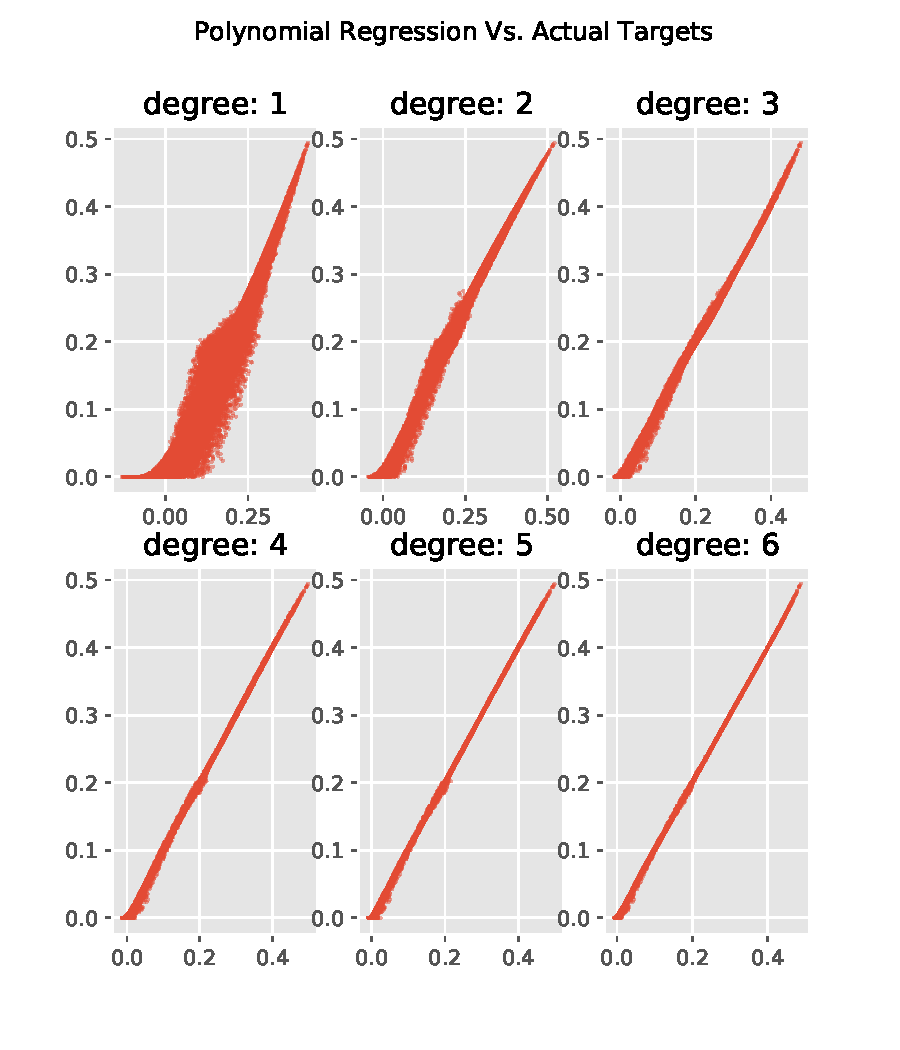
\includegraphics{Figures/polynomialEuroC.png}
\decoRule
\caption[Polynomial Regression Predictions Vs. Actual Prices]{Predicted price based on polynomial regression of varying degree}
\label{fig:PolynomialEuroC}
\end{figure}

\begin{table}[th]
\caption{In-sample validation error for european call for polynomial regression and MLPS}
\label{tab:euroPerformance}
\centering
\begin{tabular}{l l}
\toprule
\textbf{Model} & \textbf{Val. Loss} \\
\midrule
Linear Reg. & 0.000631 \\
2. degree  poly.  & 0.000069 \\
4. degree poly.  & 0.000004 \\
5. degree poly.  & 0.000002 \\
MLPs        & 0.000003\\
\bottomrule\\
\end{tabular}
\end{table}
The table is created to compare the performance for each model. The table confirms that the linear regression has a worse fit than the other models with higher capacity. The difference on the MLPs and best performing polynomial model are less than $1\cdot 10^{-6}$. The difference is negible so the fit for MLPs and polynomial regression of degree 4-6 performs all very well on the data.


%-----------------------------------
%	SUBSECTION 3
%-----------------------------------
\subsection{Model Performance}
The model performance is evaluated by MSE, RMSE, MAE and coefficient of determination, where all the measures evaluate how close the model predictions are with the actual targets. The first three measures ranges are $\mathbb{R}^+$, where the goal is to have the lowest value possible. For MSE close to 0 means that the model predictions does not differ a lot from the observed targets. The RMSE and MAE are same kind of measure, but the deviation is measured slightly different. The coefficient of determination has range $(-\infty, 1]$, where a higher value indicate a better model. Coefficient of determination provides a measure of how well observed targets are predicted by the model, based on the proportion of total variation of targets explained by the model.

\subsubsection{European Call Option}
The european call option is trained with a dataset size of 300.000 samples, $\eta=0.001$ and a batch size of 64. 

\begin{table}[th]
\caption{Prediction results for european call test data for in sample}
\label{tab:euroParRange}
\centering
\begin{tabular}{l l l l l l }
\toprule
\textbf{MSE} & \textbf{RMSE} & \textbf{MAE} & \textbf{Coefficent of Determination} \\
\midrule
0.000006 & 0.002419 & 0.0019661242 & 0.99942\\
\bottomrule\\
\end{tabular}
\end{table}



The performance measures are generally good, we see MAE, MSE and RMSE all have values less than 0.002419 from zero and a coefficient of determination 0.00058 from 1. 

\begin{figure}[th]
\centering
\includegraphics{Figures/PredictionEuroC.png}
\decoRule
\caption[MLPs Predictions Vs. Actual Prices]{Predicted price based on MLPs model}
\label{fig:MLPsEuroC}
\end{figure}

Illustration of the model fit is also provided, where the plot shows $\frac{c(S_0,K)}{K}$ predicted from the model and observed target values. The conclusion from the performance metrics is also present in the figure, where we see the model predicts close to target values over the whole range. Before moving on to pricing for american options, we investigate if polynomial regression can perform as MLPs

\begin{table}[H]
\caption{Parameter range}
\label{tab:totalEuroParRange}
\centering
\begin{tabular}{l l l l l l l }
\toprule
\textbf{Dataset} & \textbf{Moneyness} & \textbf{r} & \textbf{$\sigma$} & \textbf{T} \\
\midrule
In-Sample & 0.8-1.2 & 1\%-3\% & 0.05-0.5 & 1/252-3.0\\ 
Out-Of-Money & 0.6-0.8 & 1\%-3\% & 0.05-0.5 & 1/252-3.0\\ 
Longer Maturity & 0.8-1.2 & 1\%-3\% & 0.05-0.5 & 3-0-5.0\\ 
\bottomrule\\
\end{tabular}
\end{table}

\begin{table}[th]
\caption{Performance of predictive strength for different regression models}
\label{tab:euroPerformanceComparision}
\centering
\begin{tabular}{l l l l l l l l }
\toprule
\textbf{Model} & \textbf{Dataset} & \textbf{MSE} & \textbf{RMSE} & \textbf{MAE} & \textbf{$R^2$} \\
\midrule
Linear Reg. & In-Sample & 0.000631 & 0.025122 & 0.018264 & 0.937445\\
2. degree &  & 0.000069 & 0.008298 & 0.006136 & 0.993175\\
4. degree &  & 0.000004 & 0.002059 & 0.001282 & 0.999580\\
5. degree &  & 0.000002 & 0.001407 & 0.000864 & 0.999804\\
MLPs &  & 0.000003 & 0.001628 & 0.001337 & 0.999736\\
Linear Reg. & Out-Of-Money & 0.005772 & 0.075973 & 0.060936 & -2.377251\\
2. degree &  & 0.000767 & 0.027694 & 0.022203 & 0.551246\\
4. degree &  & 0.000944 & 0.030724 & 0.020542 & 0.447668\\
5. degree &  & 0.001812 & 0.042568 & 0.027125 & -0.060261\\
MLPs &  & 0.000005 & 0.002152 & 0.001569 & 0.997291\\
Linear Reg. & Longer Maturity & 0.002662 & 0.051593 & 0.041232 & 0.818143\\
2. degree &  & 0.001196 & 0.034577 & 0.026287 & 0.918316\\
4. degree &  & 0.003956 & 0.062894 & 0.039932 & 0.729744\\
5. degree &  & 0.012255 & 0.110702 & 0.064402 & 0.162742\\
MLPs &  & 0.000066 & 0.008138 & 0.005817 & 0.995475\\
\bottomrule\\
\end{tabular}
\end{table}


\begin{figure}[th]
\centering
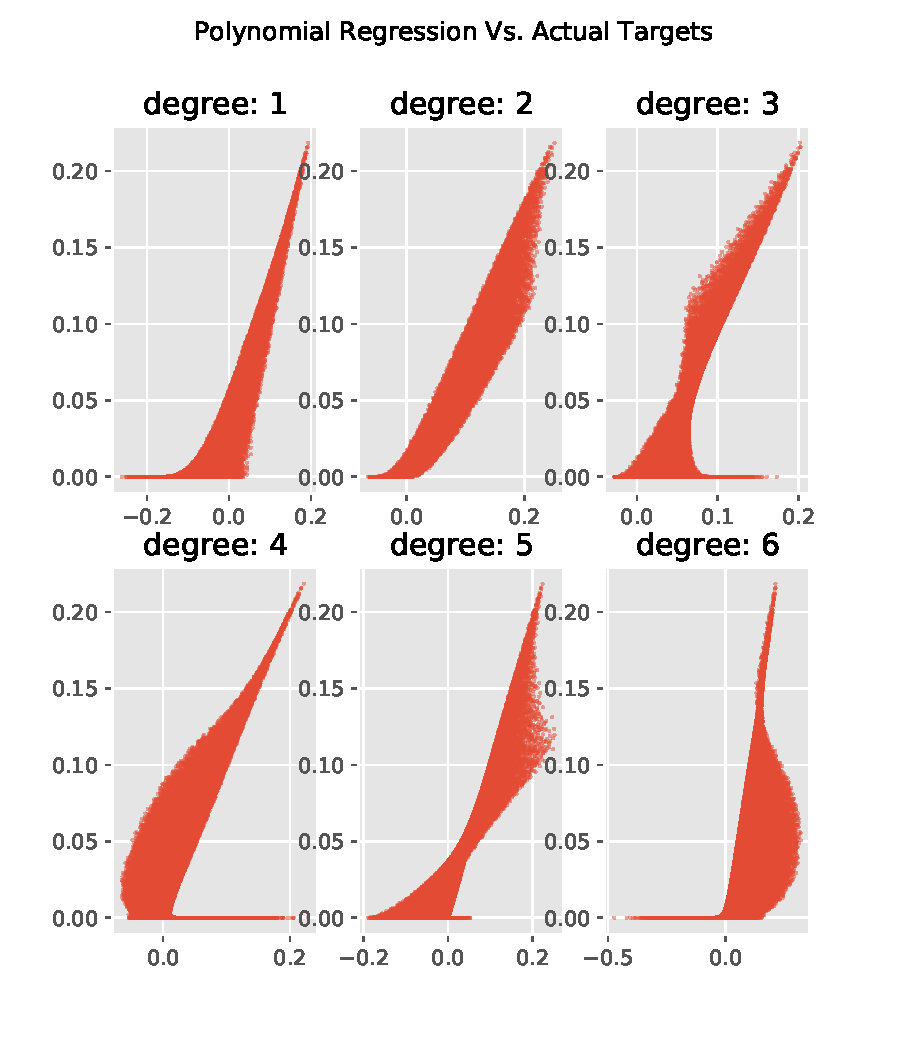
\includegraphics{Figures/polynomialOutMoneyEuroC.png}
\decoRule
\caption[Polynomial Regression Predictions Vs. Actual Prices]{Predicted price based on polynomial regression of varying degree}
\label{fig:PolynomialOutMoneyEuroC}
\end{figure}

\begin{figure}[th]
\centering
\includegraphics{Figures/PredictionOutMoneyEuroC.png}
\decoRule
\caption[MLPs Predictions Vs. Actual Prices]{Predicted price based on MLPs model}
\label{fig:MLPsOutMoneyEuroC}
\end{figure}

%\begin{figure}[th]
%\centering
%\includegraphics{Figures/PredictionLongTEuroC.png}
%\decoRule
%\caption[MLPs Predictions Vs. Actual Prices]{Predicted price based on MLPs model}
%\label{fig:MLPsEuroC}
%\end{figure}


%\begin{figure}[H]
%\centering
%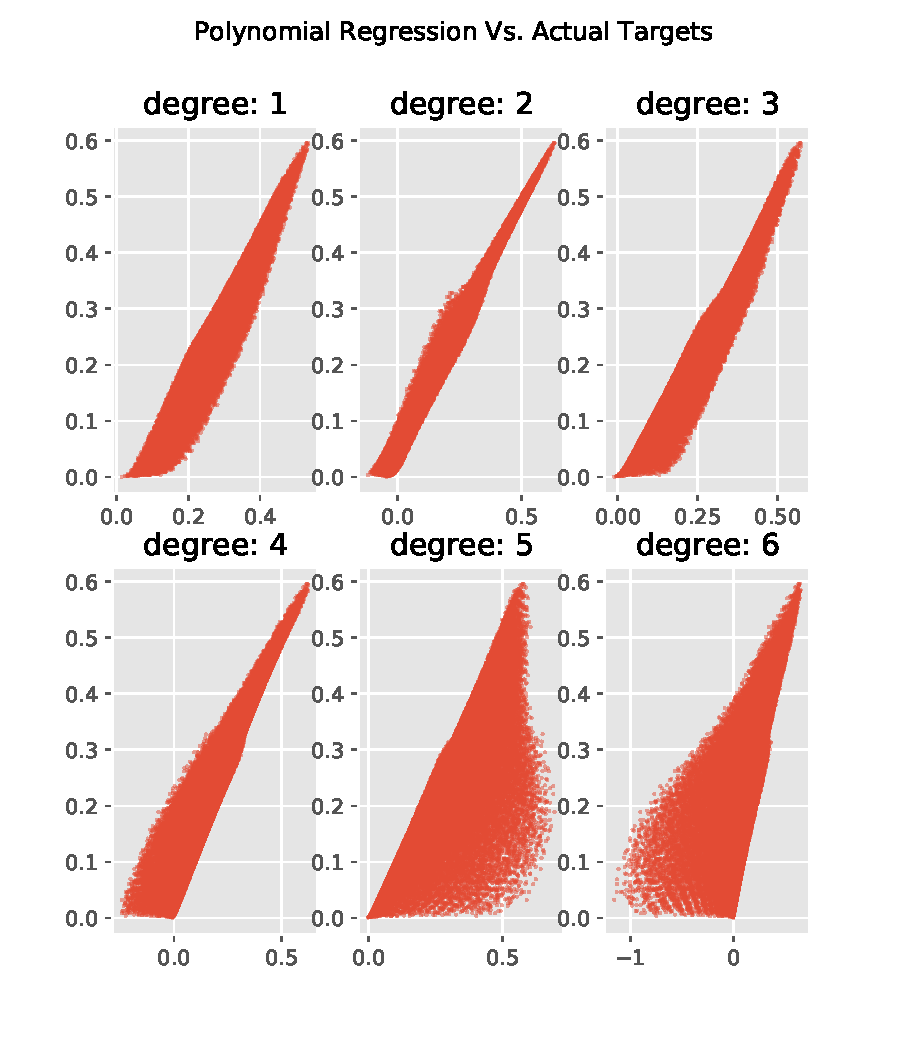
\includegraphics{Figures/polynomialLongTEuroC.png}
%\decoRule
%\caption[Polynomial Regression Predictions Vs. Actual Prices]{Predicted price based on polynomial regression of varying degree}
%\label{fig:PolynomialEuroC}
%\end{figure}


\subsubsection{American Put Option}

\begin{table}[th]
\caption{Performance of predictive strength for different regression models}
\label{tab:euroPerformanceComparision}
\centering
\begin{tabular}{l l l l l l l l }
\toprule
\textbf{Model} & \textbf{Dataset} & \textbf{MSE} & \textbf{RMSE} & \textbf{MAE} & \textbf{$R^2$} \\
\midrule
MLPs Reg. & In-Sample & 0.000002 & 0.001562 & 0.001278 & 0.999634\\
MLPs Reg. & Out-Of-Money & 0.000030 & 0.005503 & 0.003925 & 0.989674\\
MLPs Reg. & Longer Maturity & 0.000194 & 0.013922 & 0.010731 & 0.980759\\
\bottomrule\\
\end{tabular}
\end{table}

\begin{figure}[th]
\centering
\includegraphics{Figures/PredictionAmerP.png}
\decoRule
\caption[MLPs Predictions Vs. Actual Prices For American Put]{Predicted price based on MLPs model, where the targets are from the binomial model}
\label{fig:PredictionAmerP}
\end{figure}

\begin{figure}[th]
\centering
\includegraphics{Figures/PredictionOutMoneyAmerP.png}
\decoRule
\caption[MLPs Predictions Vs. Actual Prices For American Put]{Predicted price based on MLPs model, where the targets are from the binomial model}
\label{fig:PredictionOutMoneyAmerP}
\end{figure}

\begin{figure}[th]
\centering
\includegraphics{Figures/PredictionLongTAmerP.png}
\decoRule
\caption[MLPs Predictions Vs. Actual Prices For American Put]{Predicted price based on MLPs model, where the targets are from the binomial model}
\label{fig:PredictionOutMoneyAmerP}
\end{figure}

\subsubsection{American Put On Minimum of Two Assets Option}












The standard measures mean square error (MSE) and root mean square error (RMSE) shows that the MLPs increase its precision for in-sample interpolation, but for the out-of-sample datasets the decreasing error hits a plateau for 80K data samples.  


%MLPs & Out-Of-Money: 60K & 0.000075 & 0.008656 & 0.006250 & 0.956157\\
%MLPs &  & 0.000033 & 0.005702 & 0.004084 & 0.980976\\
%MLPs &  & 0.000005 & 0.002253 & 0.001770 & 0.997031\\
%MLPs &  & 0.000005 & 0.002152 & 0.001569 & 0.997291\\
%MLPs &  & 0.000006 & 0.002371 & 0.001715 & 0.996710\\


actual data samples agrees with the model for both in-sample and out-of-sample. The in-sample training is based on the parameter ranges in table \ref{tab:euroParRange}, where the out-of-sample is 60.000 simulated samples, where the moneyness lies between 0.6-0.8 and the other ranges remain the same.  Table \ref{tab:euroDataSize} shows how the validation error for in-sample and the test-error for out-of-sample datasets perform varying the number size of the training dataset. The validation error declines for increasing sample size, but the test error does not improve significantly for 100K up to 1M. The test error decreases for 100K-300K, but it increases for 300K-1M, hence we choose to work with the 300K dataset in the analysis. The 
RMSE match units - standard deviation of residuals how much spread away from mean
Coefficient of determinant metric of correlation
variation around the mean.
predictic how the regression does compared to only fitting with the mean
Does our regression fit better the data than the mean
less variation around the mean. Hence most variation is explained by the regression. some number less variation around the line vs the mean
agrees fits for most samples, but for 



The same architecture is applied to each dataset and the Adam optimizer uses minibatches of size 64.

The training algorithm is 


All the models considered had good performance on the in-sample dataset except of the too simple models linear regression and 2. degree polynomial regreesion. To test the predictive strength for the models, we test the models with out-of-sample data. Specifically we consider longer maturity and deep-out-of-money options (see table \ref{tab:totalEuroParRange})

The performance measures show that the polynomial regression that was performing better on the In-Sample dataset was due to overfitting, because the high order polynomial regression does perform poorly on out-of-sample data (see table \ref{tab:euroPerformanceComparision} and figure \ref{fig:PolynomialOutMoneyEuroC}). For the 5. order polynomial regression, we see a negative coefficient of determination, which means the model performs worse than the model with the mean as a horizontal line. This means the 5. order polynomial clearly have low predictive strength. 



We see that the 2. degree polynomial is best on most of the performance measures for our-of-sample data. Notice based on MAE for out-of-money data the 4. degree polynomial performs better than the 2. degree polynomial, but if we look at the MSE the performance is best for the 2. degree polynomial. This is due to that the two measure weight errors in different ways, where the MSE penalize large error more than the MAE. Amoung the polynomial the 2. degree polynoial regression performs best, but gets outperformed by MLPs (see also figure \ref{fig:MLPsOutMoneyEuroC}). The MLPs has high predictive strength compared to the polynomials, because it performs well also on out-of-sample dataset. The section showed how succesfully MLPs can be used in a GBM model setup for pricing european options. The MLPs is not based on a model, it can only see data. This is promising because the MLPs could also be used for actual market data or different models to learn patterns. In the coming sections we will focus on american put options and basket options, where in the basket option case the MLPs benefit for the fact that it does not increase expontially with the dimension to maintain low error compared to polynomial regression. For the american put option the MLPs regression will only be considered, because the polynomial regression have low predictive strength for the simpler european option.





The results are promosing, because the MLPs are model free in the sense, that we could have simulated out for any model, where MLPs then learn from data only. By observing this the method can be extended to real market data in fact \parencite{GasparRaquel20} have resently showed good results for a MLPs for real market data. The next section will investigate the curse of dimensionality and the application of MLPs in this context.
\parencite{FergusonRyan2018}









 
% Chapter Template

\chapter{Numerical Investigation and Discussion} % Main chapter title

\label{Chapter6} % Change X to a consecutive number; for referencing this chapter elsewhere, use \ref{ChapterX}

This chapter will empirically compare the numerical and analytical methods presented for different types of contingent claims\footnote{The interested reader can see the implementation details in appendix \ref{AppendixD}}. The underlying model will be the Black-Scholes model, because it has closed form solutions for some European options and is thoroughly researched.\\

We look at the closed form solutions to the European options compared with the binomial lattice model for pricing. The closed form solution provides a measure of how the binomial lattice model approximates European options in the Black-Scholes model. The binomial model is readily extended to American options, hence, the section also gives an indication of how the binomial model approximates the American option. The American put option is then investigated, where the different numerical methods considered are compared. The last type of option we look at is the American put minimum on two stocks option. After the numerical investigation the pricing methods and model assumptions are discussed.


%----------------------------------------------------------------------------------------
%	SECTION 1
%----------------------------------------------------------------------------------------
\section{European Options}\label{EuroOption}
European options are simple in the sense, that they can only be exercised at maturity. Throughout the previous chapters, especially chapter \ref{Chapter2} and \ref{Chapter3}, we have seen closed form solutions for the simple European and exotic European options. The binomial lattice models presented are models that can approximate European options and American options. The closed form solutions and the binomial lattice approach can be compared for European options, where a small deviation between methods for the European options indicates that the lattice approach gives reasonable prices for the American options.\\

The simplest case is the European call option, where we look at how the CRR model and the MLP II pricing model approximate the B-S call formula. Table \ref{tab:EuroCall} empirically shows that the CRR model price prediction converges toward the price from the Black-Scholes call formula, which is in line with the theoretical result for the CRR model that it converges to the Black-Scholes model. The MLP II pricing method underprices the European call option, but it performs better for this example than the CRR with 10 and 30 time-steps. Keep in mind we trained the MLP II with the CRR 100 equidistant time-steps model, therefore, we might have seen a better fit with a data set generated with $10^4$ time-steps.\\

\begin{table}[th]
\caption{CRR, MLP II, and B-S Call Formula Comparison}{Comparison of accuracy for the European call option, where the inputs are K=40, $S(0)=40$, $\sigma=0.2$, T=1, and r=0.06.}\\
\label{tab:EuroCall}
\centering
\begin{tabular}{l l l}
\toprule
\textbf{Method} & \textbf{No. Steps} & \textbf{Price} \\
\midrule
CRR & 10 & 4.316\\
& 30 & 4.369\\
& 50 & 	4.380\\
& 100 & 4.388\\
& 200 & 4.392\\
& 500 & 4.394\\
& 1000 & 4.395\\
& 10000 & 4.396\\
MLP II & & 4.370\\
Analytic form & & 4.396\\
\bottomrule\\
\end{tabular}
\end{table}

The natural extension of the CRR model is the BEG model, where it is possible to price more exotic options. Section \ref{ExoticEuro} showed some closed form solutions for exotic European options. Hence, we have a benchmark for the BEG in these special cases. We choose to look at the computation time for European put minimum with two underlying assets, which has a closed form solution. Closed form solutions make it easy to look at the trade-off between accuracy and computational cost for the BEG method. \\

\begin{table}[th]
\caption{BEG Accuracy and Speed}{Comparison of speed and accuracy for a European put min option, where the inputs are K=40, $S_1(0)=S_2(0)=40$, $\sigma_1=0.2, \sigma_2=0.3$, T=1, $\rho=0.5$,  and r=0.06. Note ms is shorthand for millisecond}
\label{tab:TradeOffEuroMin}
\centering
\begin{tabular}{l l l l}
\toprule
\textbf{Method} & \textbf{No. Steps} & \textbf{Price} & \textbf{Time: min:sec.ms} \\
\midrule
BEG & 10 & 4.248 & 0:00.003\\
& 50 & 4.341 & 0:00:097\\
& 100 & 4.352 & 0:00.591\\
& 200 & 4.358 & 0:04.121\\
& 500 & 4.361 & 0:59.337\\
& 1000 & 4.362 & 9:34.164\\
Analytic form & & 4.363 & \\
\bottomrule\\
\end{tabular}
\end{table}
Tabel \ref{tab:TradeOffEuroMin} shows that the algorithm accuracy increases with the number of equidistant time-steps, but the computational speed dramatically slows down when the time-steps increases. Therefore, for exotic options the computational costs become a factor to consider\footnote{Note the implementation is written in Python, hence, the code can be improved in terms of computational efficiency. The computations are performed on my laptop with 8GB ram and 8th Generation Intel® Core™ i5 processor}. The BEG method accuracy is also tested on the European call minimum and European call maximum for 100 time-steps, where the BEG method is within 0.13 of the analytic solution (table \ref{tab:PriceEuropean}).\\
\begin{table}[th]
\caption{BEG and Exotic European Options}{Valuation of bivariate contingent claims with K=40, $S_1(0)=S_2(0)=40$, $\sigma_1=0.2, \sigma_2=0.3$, T=1, $\rho=0.5$,  and r=0.06.}
\label{tab:PriceEuropean}
\centering
\begin{tabular}{l l l l}
\toprule
\textbf{Derivative type} & \textbf{Method} & \textbf{No. Steps} & \textbf{Price} \\
\midrule
European Call Minimum & BEG & 100 & 2.475\\
& Analytic form & & 2.483\\
European Call Maximum & BEG & 100 & 7.787\\
& Analytic form & & 7.800\\
\bottomrule\\
\end{tabular}
\end{table}
 
The above tables show that the binomial pricing model can be used for both univariate and bivariate European contingent claims. The binomial model accuracy is high for European options, hence, we expect a similar good approximation for the American option. The CRR for univariate and BEG for bivariate contingent claims will be used as benchmarks for the American options, where we investigate LSM, MLP I and MLP II pricing methods. \\

Note that the BEG is not practical for pricing multivariate contingent claims with many underlying assets, because the possible states for the stochastic processes increase exponentially. Therefore, the bivariate contingent claim is considered instead of higher dimensional basket options in section \ref{bivariateAmerPut}.
%----------------------------------------------------------------------------------------
%	SECTION 2
%----------------------------------------------------------------------------------------
\section{American Put Option}
The American put option has no analytical solution in the Black-Scholes model, thus, numerical methods are required. We present and compare the results for the LSM, MLP I and MLP II pricing methods compared to the CRR model.\\

The LSM and MLP I pricing method are almost identical, except the MLP tries to utilize deep learning to regress the expected continuation value. Both pricing methods converge to the optimal value process\footnote{See appendix \ref{Convergence}}, hence, we numerically expect that by increasing the computational burden we approach the true price. To compare the two methods we simulate $10^5$ paths for the stock under the assumption that the future price of the stock is lognormal. The LSM and MLP I pricing methods are used on the same simulated paths, but produce a different result each time due to the Monte Carlo simulations. The CRR and MLP II\footnote{Note that we talk about the model after training} are not random in the sense that the output is deterministic, because both approaches do not involve Monte Carlo simulation. For the LSM and MLP I we assume 50 equidistant exercise dates for each year, where for the CRR we use 1000 equidistant time-step for the stock.  \\

The MLP I require us to set some hyperparameters, where we choose the learning rate $\eta=0.001$, batch size of 512 and the Adam optimization algorithm. The architecture of the MLP is three layers, where the hidden layers are with 40 neurons and the output layer has one neuron. The activation functions are set to Leaky ReLU with 0.3 negative slope and the trained model is reused at each decision point by inspiration from \parencite{Lelong19}. The choices are partly inspired by the work by \parencite{Lelong19} and empirical testing. The regression in the LSM is done with a polynomial regression of degree 10. Remember the MLP II is trained with the same hyperparameters as for the European call option and the CRR with 100 time-steps is used to generate labels.\\

\begin{table}[th]
\caption{Valuation of American Put Option}{We choose the fixed parameters K=40 and r=0.06}
\label{tab:AmericanPut}
\centering
\begin{tabular}{l l l l l l l }
\toprule
\textbf{Spot} & \textbf{$\sigma$} & \textbf{T} & \textbf{CRR} & \textbf{LSM} & \textbf{MLP I} & \textbf{MLP II} \\
\midrule
36 & 0.2 & 1 & 4.487 & 4.481 & 4.364 & 4.584\\
36 & 0.2 & 2 & 4.848 & 4.846 & 4.747 & 4.649\\
36 & 0.4 & 1 & 7.109 & 7.118 & 6.919 & 7.090\\
36 & 0.4 & 2 & 8.508 & 8.514 & 8.215 & 8.487\\
38 & 0.2 & 1 & 3.257 & 3.258 & 3.217 & 3.094\\
38 & 0.2 & 2 & 3.751 & 3.748 & 3.681 & 3.638\\
38 & 0.4 & 1 & 6.154 & 6.157 & 6.075 & 6.172\\
38 & 0.4 & 2 & 7.675 & 7.695 & 7.359 & 7.605\\
40 & 0.2 & 1 & 2.319 & 2.317 & 2.292 & 2.114\\
40 & 0.2 & 2 & 2.900 & 2.896 & 2.823 & 2.779\\
40 & 0.4 & 1 & 5.318 & 5.329 & 5.180 & 5.274\\
40 & 0.4 & 2 & 6.923 & 6.934 & 6.750 & 6.839\\
42 & 0.2 & 1 & 1.621 & 1.623 & 1.599 & 1.494\\
42 & 0.2 & 2 & 2.217 & 2.224 & 2.183 & 2.167\\
42 & 0.4 & 1 & 4.588 & 4.600 & 4.538 & 4.548\\
42 & 0.4 & 2 & 6.250 & 6.269 & 6.111 & 6.197\\
44 & 0.2 & 1 & 1.113 & 1.119 & 1.094 & 1.000\\
44 & 0.2 & 2 & 1.694 & 1.700 & 1.653 & 1.678\\
44 & 0.4 & 1 & 3.954 & 3.959 & 3.931 & 3.949\\
44 & 0.4 & 2 & 5.647 & 5.669 & 5.524 & 5.649\\
\bottomrule\\
\end{tabular}
\end{table}

Table \ref{tab:AmericanPut} shows that the MLP I always predicts a lower price than the LSM, therefore, for our numerical study, the LSM seems to be better than the MLP I in terms of approximating the \textsl{"true"} price. The reference is the CRR model, which is a deterministic method. The MLP II trained with the CRR model shows high deviation from the CRR predicted price compared to LSM. The total deviation in absolute distance for the MLP II is 1.56, where LSM deviation is 0.157 for the above table containing 20 prices with different unique input parameters combinations. The MLP II is, however, better in total absolute deviation compared to the MLP I, which has a total absolute deviation of 2.078. This indicates that the MLP II, at this stage of development, is preferred over the MLP I in terms of speed and accuracy. The MLP I and LSM have uncertainty from the Monte Carlo simulation and with $10^5$ paths the standard error of the means are 0.0019 and 0.0214. The standard error\footnote{Sometimes written in short form SE} of the means are calculated by 100 samples\footnote{Denoted with n in the formulas} for the input parameters T=1, $\sigma=0.4$, $r=0.06$, $S(0)=36$, and $K=40$. The empirical distribution mean is calculated by
$$\bar{x}= \frac{1}{n}\sum_{i=1}^{n} x_i$$
and the standard error of the mean
$$\sigma_{\bar{x}}= \frac{\sigma}{\sqrt{n}} \quad where \ \sigma=\sqrt{\frac{1}{n-1}\sum_{i=1}^{n} (x_i-\bar{x})}$$
 
The histogram (figure \ref{fig:histLSMMLPI}) shows the variation in the estimates where the CRR price is the dashed black line. We see that the the MLP I has higher standard error than the LSM and the center of the distribution\footnote{Sample mean is 6.9048} is lower than the CRR price\footnote{CRR price is 7.1094}. The LSM, on the other hand, has less variability and the center\footnote{Sample mean is 7.1074} is around the CRR price. Hence in term of numerical stability, computational speed and accuracy the LSM is superior for the American put. The reason for the numerical instability for the MLP I is that the optimization algorithm is random on each run compared to the linear model\footnote{E.g. polynomial regression where the solution is exact and unique}.\\

\begin{figure}[H]
\centering
\includegraphics{Figures/histLSMMLPsI.png}
\decoRule
\caption[Histogram Price Predictions]{Predicted prices for American put option with LSM and MLP. Parameters are T=1, $\sigma=0.4$, $r=0.06$, $S(0)=36$, and $K=40$. Note CRR price is the dashed black line.}
\label{fig:histLSMMLPI}
\end{figure}

Improvements of MLP I is needed in order for the method to challenge the existing LSM, both in terms of speed and accuracy for low dimensional problem. Possible improvement of the MLP I could be conducted by a large hyperparameter tuning study. The issue with hyperparameter tuning is that it is computationally expensive. For the MLP I the hyperparameter tuning needs to be searched at every decision point. Another type of network could also be considered, e.g. recurrent neural network. The inferior results from the MLP I to the LSM show that some work still needs to be done. We choose not to consider MLP I and LSM for the next section, because of the poor results from the MLP I pricing method in this section.\\
%----------------------------------------------------------------------------------------
%	SECTION 3
%----------------------------------------------------------------------------------------
\section{American Put Minimum on two Assets Option}\label{bivariateAmerPut}
There are many exotic American options to consider, but we choose to focus on the American put minimum on two stocks option, because MLP II is trained to predict prices on this specific option. The other advantage is that we have the deterministic method BEG for the bivariate contingent claim, hence, the MLP II can easily be compared, both for accuracy and speed.\\

First, we look at the computational cost for the BEG method by increasing the number of time-steps. By looking at table \ref{tab:TradeOffAmerMin} it is clear that the computational time is dependent on the number of time-steps. We know from the discussion in section \ref{EuroOption} that the accuracy increases by increasing the number of time-steps. Weighting the computational cost and accuracy we choose to use the BEG method as reference price with 500 time-steps. Note, that when we generated the labels for the MLP II pricing method we used 50 equidistant time-steps. The reason for using 50 time-steps is that we simulated 300.000 data points, which is a computational heavy task. A MLP II model trained with 500 time-steps would probably predict the price from the BEG method with 500 steps better, but it was not computationally feasible. This creates an expectation that the option priced with MLP II will have a bias price and therefore, we will also include the BEG with 50 time-steps in the comparison.\\

\begin{table}[th]
\caption{BEG for the American Bivariate Contingent Claim}{Comparision of speed for the American put minimum on two assets option, where the inputs are K=40, $S_1(0)=S_2(0)=40$, $\sigma_1=0.2, \sigma_2=0.3$, T=1, $\rho=0.5$  and r=0.06. Note ms is shorthand for millisecond}
\label{tab:TradeOffAmerMin}
\centering
\begin{tabular}{l l l l}
\toprule
\textbf{Method} & \textbf{No. Steps} & \textbf{Price} & \textbf{Time: min:sec.ms} \\
\midrule
BEG & 10 & 4.524 & 00:00.006\\
& 50 & 4.594 & 00:00.250\\
& 100 & 4.602 & 00:01.837\\
& 200 & 4.605 & 00:14.025\\
& 500 & 4.608 & 03:35.039\\
& 1000 & 4.609 & 28:32.584\\
MLP II &  & 4.426 & 00:00.0003\\
\bottomrule\\
\end{tabular}
\end{table}

Table \ref{tab:TradeOffAmerMin} shows that the price for the American put minimum is greater than the European put minimum from table \ref{tab:TradeOffEuroMin}. Additionally, it is clear that the computational time increases for the American option, because we have to compare intrinsic value and expected continuation value at each node. Both results are good sanity checks.\\

For visualization we plot the BEG50, BEG500, and MLP II for varying spots with fixed K=40, $\sigma_1=0.2$, $\sigma_2=0.3$, T=1, $\rho=0.5$,  and r=0.06. The figure shows that the BEG500\footnote{BEG method with 500 time-steps} and BEG50 are close to each other. The total absolute deviation is 0.142 for the 21 prices, which shows that the BEG50 is suffient for training our MLP. The total absolute deviation for the MLP II with the BEG500 is 3.716 and with the BEG50 3.713. This is depicted in figure \ref{fig:BEGMLPII}, where the MLP underprices the option for the in-sample domain with varying spot. To compare the computational speed the MLP II took around 00:00.000349 to generate one price, which is considerable faster than the BEG model with 10 time-steps. Hence, we see that we loose some accuracy with the MLP II, but the pricing method is fast. 

\begin{figure}[H]
\centering
\includegraphics{Figures/compareBEGMLPsII.png}
\decoRule
\caption[Compare BEG and MLP II]{Scatter plot of predicted prices for American put minimum on two assets option with BEG and MLP II. Parameters are T=1, $\sigma_1=0.2$, $\sigma_2=0.3$, $r=0.06$, $K=40$ and $\rho=0.5$. Note BEG is showed for 50 time-steps and 500 time-steps.}
\label{fig:BEGMLPII}
\end{figure}

The MLP might provide a better estimate by simulating more data samples and make the model more complex, but our hyperparameter tuning study was not conclusive on this point. Hyperparameter tuning could also be further investigated, e.g. looking at depth and width of the network. The real power of pricing with MLP II is when the computational burden becomes an issue for fast pricing. 

%----------------------------------------------------------------------------------------
%	SECTION 4
%----------------------------------------------------------------------------------------
\section{Discussion of Pricing Methods}
The idea behind using neural networks instead of the linear model, is that the neural networks scale better for high dimensional problems. We have only considered univariate and bivariate contingent claims, because in these cases we have a deterministic alternative in the binomial lattice models. This gives a good indication of how the model predicts. Besides, if the model does not perform well for low dimensional problems, we would not expect the model to be any better for more complex multivariate contingent claims.\\

Remember, the binomial lattice model also has its limitations in terms of computational resources, because the computational burden scales exponentially with the number of underlying risky assets\footnote{The same can be said about the PDE methods}. The LSM is versatile and can be used for most derivatives, because it relies on Monte Carlo simulation and regression. For considering multivariate contingent claims the LSM is readily useful, but the linear model for regression suffers the curse of dimensionality for basket options with many underlying risky assets. We have in mind that a neural network does not suffer from the curse of dimensionality, hence, the method, compared to the linear model, has advantages when considering multivariate contingent claims. The idea of neural network should work in theory\footnote{Universal approximation theorem for MLP}, but the numerical results shown in this chapter are not satisfying for the MLP I in the univariate case.\\

The MLP II is somewhat better, but it still relies on existing option pricing methods or real market data. Therefore, it does not solve the curse of dimensionality for basket options with many underlying assets. The MLP II however, has the advantage of the increased speed after training, which could be beneficial in some circumstances. The MLP could also be used on real data and it is versatile enough to capture the volatility shew\footnote{Explanation below in section "Discussion of the Black-Scholes model"} for equity options. One drawback is that there should be enough data samples, which is relevant if the method is used on real market data. Another drawback is that the trained model would need to be calibrated regularly, because financial scenarios can change dramatically, e.g. the financial crisis in 2007-2009.\\

In the training phase of the neural networks the derivatives of the model parameters are used for minimizing the loss function. The derivatives are calculated efficiently with backpropagation, which is important for risk management. Potentially, the neural networks can speed up the risk management of the derivative books and give real time risks. Deep learning for risk management is investigated in \parencite{AntoineSavine}. It should be mentioned, that the above-mentioned methods cannot only be used for equity options, the LSM is e.g. widely used for fixed income\footnote{E.g. Libor Market Model}.\\

The results from the MLP I were a bit discouraging, because it was inferior to the LSM. The computational cost is higher for the MLP I for low dimensional problems, hence, an accuracy on the same level as for the LSM would make it attractive to investigate for higher dimensional problems. One explanation could be wrong hyperparameters for the model, which would require a time consuming hyperparameter search. The grid search might have its shortcomings in this aspect, because it requires some knowledge about possible well-suited hyperparameters for the optimal stopping problem. A random search or Bayesian search could be beneficial in this aspect, but it would also require many computational resources.\\

The MLP II lack some precision compared to LSM for the univariate contingent claim. For the bivariate the MLP II again showed a loss of accuracy, but showed additional speed. A larger hyperparameter study could also be conducted here, a different method to generate labels or a bigger data set could have been sampled. E.g. the article \parencite{FergusonRyan2018} shows good result for an European basket option with 6 underlying assets by simulating a data set of 500M samples. 

%----------------------------------------------------------------------------------------
%	SECTION 5
%----------------------------------------------------------------------------------------
\section{Discussion of the Black-Scholes model}
For pricing we utilize the Black-Scholes theory, where we assume constant volatility, the interest rate is constant through time, and future stock prices are lognormal distributed. It is well-known that the volatility is not constant, in fact, it depends on the maturity and strike. The dependency on strike and maturity can be modeled with a volatility surface. Looking only at one dependency the implied volatility for equity options is a decreasing function of the strike over spot $\frac{K}{S(0)}$ for real data (p. 458 \parencite{Hull}). This phenomenon is known as volatility shew for equity options. \\

A possible reason for the volatility shew is that investors are more concerned with falling stock prices than rising prices, hence, the volatility is instantaneously negatively correlated with the stock price. To overcome the issue about assuming constant volatility, a model with stochastic variance can be considered. The model becomes more complex with an extra stochastic variable, where for simplicity we mention the two factor Heston model. The basic model is given by the stock follow the SDE:
$$dS(t)=\alpha S(t) dt + \sqrt{V(t)} S(t) dW_S(t)$$
And the stochastic variance process $V(t)$ is the solution to the SDE:
$$dV(t)=a(\theta - V(t))dt + \epsilon \sqrt{V(t)} dW_V(t) \quad where \ a>0,\theta>0, \epsilon>0, \ and \ V(0)>0$$
Where $W_S(t)$ and $W_V(t)$ have correlation $\rho$. The interpretation of the constants is:
\begin{enumerate}
\item[•] $\theta$ is long run average price variance
\item[•] a is the rate which $V(t)$ reverts to $\theta$
\item[•] $\epsilon$ is the volatility of the volatility
\end{enumerate} 
The implication of $\epsilon$ is that $V(t)$ is more volatile when volatility is high. The correlation between the stock and variance process is often modeled with a negative correlation. The negative correlation between the two processes displays the real market phenomenon of volatility shew for equity options, because when the stock price drops, volatility increases. Assuming stochastic volatility the Heston model overcomes the issue with volatility shew. Another model trying to solve the non-constant volatility is e.g. "Constant Elasticity of Variance model", but there are numerous others\footnote{E.g "Merton's Mixed Jump-Diffusion Model" and "Variance-Gamma Model"}. \\

The constant risk-free interest rate through time assumption can also be discussed, because the interest rate is not constant for real market behavior. We did not investigate the American call, because it coincides with the European call for positive interest rate. Today's market interest rates are negative for the Eurozone, which was probably unheard before the last decade's financial events. Therefore, the decision to assume positive constant interest rate through time is set for convenience.\\

The Black-Scholes model assumes that the underlying risky assets evolves as a GBM, where the distribution of possible stock prices at the end of any interval is lognormal. The model is convenient, because the GBM has a analytical solution\footnote{SDE does not always have a analytical solution}. If we wanted to investigate arithmetic mean basket option the Bachelier model would be more convenient, because the future stock price is normal distributed. 
\begin{equation*}
dS_i=\sigma_i dW_i
\end{equation*}
This assumption would simplify the pricing problem of arithmetic basket options, because the sum of normals provides a multivariate normal distribution. The basket option problem in the Bachelier is then essentially one dimensional. This is similar to the the geometric mean basket option for the Black-Scholes model (section \ref{GeoBasket}). A disadvantage with the Bachelier model is that it can lead to negative stock values, which is not realistic.\\

The Black-Scholes model has some drawbacks where you can question the assumptions, but the model is convenient to use for comparison of pricing methods. By above discussion, we stress that we do not necessarily believe that the Black-Scholes model is the true model for real market behavior. The purpose is rather to investigate pricing methods in a convenient model.


% Chapter Template

\chapter{Conclusion and Further Investigation} % Main chapter title

\label{Chapter7} % Change X to a consecutive number; for referencing this chapter elsewhere, use \ref{ChapterX}

%----------------------------------------------------------------------------------------
%	SECTION 1
%----------------------------------------------------------------------------------------

\section{Conclusion}

%-----------------------------------
%	SECTION 2
%-----------------------------------
\section{Further Investigation}


%\include{Chapters/Chapterinfo}
%----------------------------------------------------------------------------------------
%	THESIS CONTENT - APPENDICES
%----------------------------------------------------------------------------------------

\appendix % Cue to tell LaTeX that the following "chapters" are Appendices

% Include the appendices of the thesis as separate files from the Appendices folder
% Uncomment the lines as you write the Appendices

% Appendix A

\chapter{Stochastic Calculus and Probability Theory} % Main appendix title

\label{AppendixA} % Change X to a consecutive letter; for referencing this appendix elsewhere, use \ref{AppendixX}

\begin{theorem}\label{Ito}
\textbf{Itô's formula multidimensional} Let the n-dimensional process X have dynamics given by:
\begin{align}
dX(t)=\mu(t)dt+\sigma(t)dW(t)
\end{align}
Then the process $f(t,X(t))$ has stochastic differential given by:
\begin{equation}
\begin{split}
df(t,X(t))=\frac{\partial f(t,X(t))}{\partial t}  dt + \sum_{i=1}^{n} \frac{\partial f(t,X(t))}{\partial x_i}  dX_i(t) + \frac{1}{2} \sum_{i,j=1}^{n} \frac{\partial^2 f(t,X(t))}{\partial x_i \partial x_j}  dX_i(t)dX_j(t)  
\end{split}
\end{equation}
Note: \[ dW_i(t) \cdot dW_j(t)= \begin{cases} 
      \rho_{ij}dt & \textit{For correlated Weiner processes} \\
      0 & \textit{For independent Weiner processes} \\
   \end{cases}
\]
\null \hfill (p. 58-60 \parencite{finKont})
\end{theorem}

\begin{theorem}\label{MRT}
\textbf{The Martingale Representation Theorem} 
Let W be a k-dimensional Wiener process, and assume that the filtration is defined by:
$$\mathcal{F}_t=\mathcal{F}_t^W \quad t\in [0,T]$$
Let M be any $\mathcal{F}_t$-adapted martingale. Then there exist uniquely determined $\mathcal{F}_t$-adapted processes $h_1, \ldots, h_k$ such that M has the representation
$$M(t)=M(0) + \sum_{i=1}^{k} \int_{0}^{t} h_i(s)dW_i(s) \quad t \in [0,T]$$
if the martingale M is square integrable, then $h_1, \ldots, h_k$ are in $L^2$\\
\null \hfill (p. 161 \parencite{finKont}).
\end{theorem}

\begin{theorem}\label{Girsanov}
\textbf{The Girsanov Theorem} 
Assume the probability space $(\Omega, \mathcal{F}, P, (\mathcal{F}_t^{\bar{W}})_{t \in [0,T]})$ and let the Girsanov kernel $\phi$ be any d-dimensional adapted column vector process. Choose a fixed T and define the process L on $[0,T]$ by:\\
$dL_t=\phi(t)^T\cdot L_t d\bar{W}_t^P$\\
$L_0=1$.\\
Assume that $E^P[L_T]=1$ and define the new probability measure $Q$ on $\mathcal{F}_T$ by:\\
$$L_T=\frac{dQ}{dP} \quad on \ \mathcal{F}_T$$
Then
\begin{align}
d\bar{W}(t)=\phi(t)dt + dW(t)
\end{align}
Where $W(t)$ is the Q-Wiener process and $\bar{W}(t)$ is the P-Wiener process.\\
\null \hfill (p. 164 \parencite{finKont})
\end{theorem}

\begin{theorem}\label{ConverseGirsanov}
\textbf{The Converse of the Girsanov Theorem} Let $\bar{W}$ be k-dimensional standard P-Wiener process (i.e. zero drift and unit variance independent components) on $(\Omega,\mathcal{F}, P, (\mathcal{F}_t^{\bar{W}})_{t \in [0,T]})$. Assume that there exits a probability measure $Q$ such that $Q<<P$ on $\mathcal{F}_T^{\bar{W}})$. Then there exists an adapted process $\phi$ such that the likelihood process L has dynamics
\begin{align*}
dL(t)=L(t)\phi^T(t)d\bar{W}(t)\\
L(0)=1
\end{align*}
\null \hfill (p. 168 \parencite{finKont})
\end{theorem}

\theoremstyle{definition}
\begin{definition}{\textbf{Stopping time}:}\label{StoppingTime}
A random variable $\tau:\Omega \to [0,\infty]$ is called a Markov time if 
$$(\tau \leq t)\in \mathcal{F}_{t} \quad \forall t \geq 0 $$
A Markov time is called a stopping time if $\tau<\infty$ P-a.s.\\
\null \hfill (p. 27 \parencite{Shiryaev06})
\end{definition}


\theoremstyle{definition}
\begin{definition}{\textbf{Snell envelope}}\label{snellEnvelope}
Consider a fixed process Y.
\begin{enumerate}
\item[•] We say that a process X dominates the process Y if $X_n \geq Y_n \ P-a.s. \ \forall n$.
\item[•] Assuming that $E[Y_n] < \infty  \ \forall n \leq T$, the Snell envelope S, of the process Y is defined as the smallest supermartingale dominating Y. More precisely: S is a supermartingale dominating Y, and if D is another supermartingale dominating Y, then $S_n\leq D_n \ P-a.s. \ \forall n$.
\end{enumerate}
\null \hfill (p. 380 \parencite{Bjork19})
\end{definition}

\begin{theorem}\label{SnellEnvelopeTheorem}
\textbf{The Snell Envelope Theorem} The optimal value process V is the Snell envelope of the gain process G.\\
\null \hfill (p. 381  \parencite{Bjork19})
\end{theorem}

% Appendix Template

\chapter{Mathematical definitions} % Main appendix title

\label{AppendixB} % Change X to a consecutive letter; for referencing this appendix elsewhere, use \ref{AppendixX}

\theoremstyle{definition}
\begin{definition}{Orthogonal vectors: }\label{OrthogonalVec}
Two vectors $\overrightarrow{a}$ and $\overrightarrow{b}$ are orthogonal, if their dot product is 0:
$$\overrightarrow{a} \cdot \overrightarrow{b} = 0$$
We will use the notation:
\begin{equation}
\begin{split}
\overrightarrow{a} \bot \overrightarrow{b}
\end{split}
\end{equation}
\end{definition}
%% Appendix Template

\chapter{Binomial Lattice Model} % Main appendix title

\label{AppendixC} % Change X to a consecutive letter; for referencing this appendix elsewhere, use \ref{AppendixX}

\section{Moment Matching CRR}\label{CRRMM}
In the CRR the stock multiplication factor for up and down movement is chosen to match the two first moments of the lognormal distribution. By matching the first moments the underlying discrete binomial stochastic process for the stock converge toward the continuous time lognormal distribution for sufficient large equidistant time-steps N. Hence the CRR model will coincide with the Black-Scholes model.\\

The SDE for the Black Scholes under the equivalent martingale measure Q:
$$dS(t)=rS(t)dt + \sigma S(t) dW(t)$$
Using Itô's lemma:
\begin{equation}\label{lnGBM}
d\ln(S(t)))=(r-\frac{1}{2}))t + \sigma W_t
\end{equation}
The solution of equation \ref{lnGBM} is then:
$$S(t)=S(0)\exp\bigg((r-\dfrac{1}{2}\sigma)t+ \sigma W(t) \bigg)$$
Note that $W(t)\sim \mathcal{N}(0,t)$ implies:
$$\ln(\dfrac{S(t)}{S(0)}) \sim \mathcal{N}((r-\dfrac{1}{2}\sigma^2)t, \sigma^2 t)$$
The two first moments for the lognormal distribution is then:
\begin{equation}\label{lnMoments}
\begin{split}
E[\dfrac{S(t)}{S(0)}]=\exp(rt)\\
E[(\dfrac{S(t)}{S(0)})^2]=\exp(t\cdot (2r + \sigma^2))
\end{split}
\end{equation}
The above derivation can be used for any time interval.\\

The binomial lattice model has two discrete outcomes from each state, hence the moments are:
\begin{equation}\label{binMoments}
\begin{split}
E[\dfrac{S(t_{n+1})}{S(t_{n})}]=u \cdot Q(\dfrac{S(t_{n+1})}{S(t_{n})} = u) + d \cdot Q(\dfrac{S(t_{n+1})}{S(t_{n})} = d) = u \cdot q + d \cdot (1-q)\\
E[(\dfrac{S(t_{n+1})}{S(t_{n})})^2]=u^2 \cdot q + d^2 \cdot (1-q)
\end{split}
\end{equation}
We match the moments (equations \eqref{lnMoments} and \eqref{binMoments}) and get two equations with two unknowns, where the time-step is chosen to be $\Delta t$
\begin{align*}
\exp(r \Delta t)=u \cdot q + d \cdot (1-q) \quad (i)\\
\exp(\Delta t \cdot (2r + \sigma^2))=u^2 \cdot q + d^2 \cdot (1-q) \quad (ii)
\end{align*}
Multipling $(i)$ with u+d and recognizing $(ii)$:
\begin{align*}
(u+d)\exp(r \Delta t)&=u^2 \cdot q + d^2 \cdot (1-q) + ud\\
\Rightarrow (u+d)\exp(r \Delta t)&\overset{(ii)}{=}\exp(\Delta t \cdot (2r + \sigma^2)) + u d
\end{align*}
Remember we choose $u= \frac{1}{d}$ hence we arrive at a quadractic equation by some algebra
\begin{align*}
u^2 - u\bigg(\exp(-r \Delta t) + \exp(\Delta t(r+\sigma^2))\bigg)+1=0
\end{align*}
We are interesed in that the binomial model converge toward the Black-Scholes model, hence we are looking at small time increment $\Delta t$. This justify the Taylor approximation of the exponential function around zero.
\begin{align*}
\exp(r \Delta t + \sigma^2 \Delta t) \approx 1 + (r+\sigma^2)\Delta t + O(t^2)
\end{align*}
By Taylor approximation we arrive at a simpler quadratic equation:
\begin{equation*}
u^2-u(2+\sigma^2 \Delta t) + 1 = 0
\end{equation*}
Solving the quadractic equation above gives
\begin{align*}
u&=1+\dfrac{1}{2} \sigma^2 \Delta t \pm  \dfrac{\sqrt{(2+\sigma^2 \Delta t)^2 - 4}}{2}\\
&=1+\dfrac{1}{2} \sigma^2 \Delta t \pm  \dfrac{\sqrt{(4+\sigma^4 \Delta t^2 + 4 \sigma^2 \Delta t - 4}}{2}\\
&=1+\dfrac{1}{2} \sigma^2 \Delta t \pm \frac{1}{2} \sigma \sqrt{\Delta t} \sqrt{\sigma^2 \Delta t + 4}\\
&\approx 1+\dfrac{1}{2} \sigma^2 \Delta t \pm \sigma \sqrt{\Delta t}\\
&\approx \exp(\pm \sigma \sqrt{\Delta t})\\
\end{align*}

%----------------------------------------------------------------------------------------
%	BIBLIOGRAPHY
%----------------------------------------------------------------------------------------




\printbibliography[heading=bibintoc]

%----------------------------------------------------------------------------------------

\end{document}  








Batch normalization\\
Important to standardize the covariates. And highly correlated covariates should be trimmed down.
It is also a good idea to standardize the hidden covariates as well. This is called batch normalization and can accelarate the training of a network considerably.\\

It is recommended to use batch normalization  in combination with dropout. \\


By using a dynamic programming argument with three strategies:
\begin{enumerate}
\item[•] Use optimal stopping strategy $\hat{\tau}_t$
\item[•] Stop immediately
\item[•] Wait one time-step h and then use optimal stopping strategy $\hat{\tau}_{t+h}$
\end{enumerate}

We will see in the American put section why these two propositions are useful. 

By following the arguments in section 25 in \parencite{Shiryaev06}, we arrive at two important propositions for numerically evaluating American options.

\begin{proposition}{\textbf{variational inequalities}}\label{varInEq}
Given enough regularity, the optimal value function is characterized by the following relations:
\begin{equation}
\begin{split}
V(T,x)=\Phi(T,x)\\
V(t,x)\geq \Phi(t,x) \quad \forall (t,x)\\
\bigg(\frac{\partial}{\partial t} + \mathbb{A}\bigg)V(t,x) \leq 0 \quad \forall (t,x)\\
\max\bigg\{V(t,x) - \Phi(t,x), \bigg(\frac{\partial}{\partial t} + \mathbb{A}\bigg)V(t,x) \bigg\} = 0 \quad \forall (t,x)\\
\textsl{Where $\mathbb{A}$ is the Itô operator:}\\
\mathbb{A}f(t,x) =  \mu(t,x) \frac{\partial f(t,x)}{\partial x} + \frac{1}{2} \sigma^2(t,x) \frac{\partial^2 f(t,x)}{\partial x^2}
\end{split}
\end{equation}
(see p. 344 \parencite{finKont})
\end{proposition}

\begin{proposition}{\textbf{Free boundary value problem}}\label{freeBoundary}
Assuming enough regularity, the optimal value function satisfies the following parabolic equation
\[ \begin{cases} 
      \frac{\partial V(t,x)}{\partial t}(t,x) + \mu(t,x) \frac{\partial V(t,x)}{\partial x}(t,x) + \frac{1}{2}\sigma^2(t,x)\frac{\partial^2 V(t,x)}{\partial x^2}=0 & (t,x)\in C \\
     V(t,x)=\Phi(t,x)  & (t,x)\in \partial C \\
   \end{cases}
\]
Where C is the continuation region defined by:
$$C=\{(t,x): V(t,x)>\Phi(t,x) \}$$
(see p. 343-344 \parencite{finKont})
\end{proposition}

The two propositions can be used to value american put options numerically, but we will take an different approach in this thesis.
So for practical use there are three strategies to find the fair price for the option:
\begin{enumerate}
\item[•] Solve the free boundary free problem numerically (see \ref{freeBoundary})
\item[•] Solve the variational inequalities numerically (see \ref{varInEq})
\item[•] Approximate the Black-Scholes model by a binomial model and compute the exact binomial American put price.\\
(p. 347 \parencite{finKont})
\end{enumerate}

At maturity the cash flow from the option is the same as for an European put option, hence the cash flow from each path is $G(S(T))=max(K-S_T,0)$. We use the notation $G(S(\tau_{t+1}))$ denote the path of cash flows generated by the option condition on the option not being exercised before t and the option holder follow the optimal stopping strategy for all s, $t<s\leq T$.
(inspired by \parencite{lsm} p. 121). The continuation value is given by:
\begin{equation}\label{continuation-value}
\begin{split}
F(\omega; t_n)=E^Q[\sum_{j=n+1}^N \exp(-\int_{t_n}^{t_j} r(\omega,s) ds) G(S(\tau_{t+1})) |\mathcal{F}_{t_k}]
\end{split}
\end{equation}
where $r(\omega,t)$ is risk free interest rate, and the $\mathcal{F}_{t_k}$ is the filtration at time $t_k$.\\

We get the optimal stopping strategy by comparing thr continuation value with the intrinsic value at each time step. By working backward in time until the initialization of the option, we have approximated the the optimal stopping times and the cash flows associated with exercising at the optimal stopping times

To estimate the condition expectation in equation \ref{continuation-value}, we regres with the basis functions taking on the underlying asset for the option being the independent variable:
 \parencite{lsm}.